\documentclass[12pt,a4paper]{report}

%==============================================================================
% PREAMBLE AND PACKAGES (Aligned with CEK / KTU B.Tech Project Format)
%==============================================================================
\usepackage{graphicx}
\usepackage{amsmath}
\usepackage{fancyhdr}
\usepackage{cite}
\usepackage{a4wide}
\usepackage{float}
\usepackage{epsfig}
\usepackage{longtable}
\usepackage{enumerate}
\usepackage{afterpage}
\usepackage{multirow}
\usepackage{ragged2e}
\usepackage{gensymb}
\usepackage{amsfonts} 
\usepackage[left=3.5cm,top=1.5cm,right=3cm,bottom=3cm]{geometry}
\usepackage{setspace}           
\usepackage{txfonts}
\usepackage{standalone}
\usepackage{tikz}
\usepackage{fontawesome5}
\usetikzlibrary{calc, shapes.geometric, arrows, arrows.meta, positioning, fit, backgrounds, shadows, tikzmark}

% Color definitions for TikZ diagrams (Clinical Deep Navy, Ocean Blue & Cyan Palette)
\definecolor{lavenderDark}{RGB}{15, 44, 89}
\definecolor{lavenderDeep}{RGB}{10, 28, 58}
\definecolor{lavenderMedium}{RGB}{29, 78, 158}
\definecolor{lavenderLight}{RGB}{240, 246, 255}
\definecolor{lavenderBorder}{RGB}{180, 205, 237}
\definecolor{lavenderAccent}{RGB}{2, 132, 199}
\definecolor{prismNavy}{RGB}{15, 44, 89}
\definecolor{prismBlue}{RGB}{29, 78, 158}
\definecolor{prismTeal}{RGB}{13, 148, 136}
\definecolor{prismMint}{RGB}{236, 253, 245}
\definecolor{prismGold}{RGB}{217, 119, 6}
\definecolor{prismDark}{RGB}{15, 23, 42}
\definecolor{prismLight}{RGB}{248, 250, 252}
\definecolor{prismIndigo}{RGB}{30, 58, 138}
\definecolor{prismSlate}{RGB}{100, 116, 139}
\definecolor{statusFail}{RGB}{220, 38, 38}
\definecolor{cInput}{RGB}{241, 245, 249}
\definecolor{cStem}{RGB}{224, 242, 254}
\definecolor{cStage1}{RGB}{209, 250, 229}
\definecolor{cStage2}{RGB}{254, 243, 199}
\definecolor{cStage3}{RGB}{254, 226, 226}
\definecolor{cStage4}{RGB}{207, 250, 254}
\definecolor{cHead}{RGB}{219, 234, 254}
\definecolor{cOutput}{RGB}{255, 228, 230}
\definecolor{cDeliverable}{RGB}{204, 251, 241}

\usepackage{subfiles}
\usepackage{adjustbox}
\usepackage{tcolorbox}
\tcbuselibrary{skins}

\newcommand{\Usefont}[1]{\fontfamily{#1}\selectfont}

\usepackage{lscape}
\linespread{1.5}

\usepackage{url}
\usepackage{subcaption}
\usepackage[intoc, english]{nomencl}
\usepackage[nottoc]{tocbibind}
\usepackage{booktabs}
\usepackage{array}
\usepackage{tabularx}
\usepackage{hyperref}

\hypersetup{
    plainpages=false,
    pdfpagelabels=true,
    colorlinks=true,
    linkcolor=black,
    citecolor=black,
    urlcolor=black,
    pdftitle={Ear Disease Detection from Otoscopic Images Using Robust Deep Learning Models},
    pdfauthor={Mohammad Salman, Jithin Joseph, Punya A J, Sana Azeez}
}

% Spacing and line-breaking settings to prevent overflow and overfull hboxes
\setlength{\headheight}{15pt}
\hyphenpenalty=1000
\tolerance=2000
\emergencystretch=2.5em

\bibliographystyle{IEEEtran}
\renewcommand{\bibname}{References}

% Figure search path
\graphicspath{{figures/}{diagrams/}{./}}

%==============================================================================
% METADATA DEFINITIONS (Project Group & CEK)
%==============================================================================
\gdef \title{EAR DISEASE DETECTION FROM OTOSCOPIC IMAGES USING ROBUST DEEP LEARNING MODELS}
\gdef \shorttitle{Ear Disease Detection from Otoscopic Images}

\gdef \authorA{MOHAMMAD SALMAN}
\gdef \rollnoA{KNP23CS076}

\gdef \authorB{JITHIN JOSEPH}
\gdef \rollnoB{KNP23CS062}

\gdef \authorC{PUNYA A J}
\gdef \rollnoC{KNP23CS087}

\gdef \authorD{SANA AZEEZ}
\gdef \rollnoD{KNP23CS092}

\gdef \acadyear{2026--2027}
\gdef \submonth{October 2026}
\gdef \month{October 2026}
\gdef \date{28-10-2026}
\gdef \dept{Computer Science and Engineering}
\gdef \deptabbr{Dept.\ of CSE}
\gdef \degree{Bachelor of Technology}
\gdef \branch{Computer Science and Engineering}
\gdef \college{College of Engineering Karunagappally}
\gdef \collegeplace{Kollam}
\gdef \collegetown{Karunagappally}

\gdef \guide{Mrs. Shameena N}
\gdef \guidedes{Assistant Professor}
\gdef \coordinator{Dr. Leena Silvoster}
\gdef \coordinatordes{Associate Professor}
\gdef \semcordinatorA{Dr. Leena Silvoster}
\gdef \semcordinatorAdes{Associate Professor}
\gdef \hod{Dr. Smitha P}
\gdef \hoddes{Associate Professor and HOD}

% Individual candidate credentials (defined by wrapper files main_salaman.tex, etc.)
% When compiling main.tex directly, candidateName is undefined so the second individual certificate is omitted.

%==============================================================================
% DOCUMENT BODY
%==============================================================================

\begin{document}

%------------------------------------------------------------------------------
% FRONT MATTER
%------------------------------------------------------------------------------
\hypersetup{pageanchor=false}
%==================================coverpage.tex================================

\thispagestyle{empty}
\begin{titlepage}
\subfile{design_cover}
	\begin{center}\fontfamily{ptm}\selectfont
		{\Large \bfseries \title \par}
		\vspace*{12pt}
		{\large \Usefont{pzc}
			A PROJECT REPORT \par
			\vspace*{5pt}
			Submitted to the APJ Abdul Kalam Technological University \par
			\vspace*{5pt}
			in partial fulfillment of requirements for the award of degree\par}
		\vspace*{8pt}
		{\large \bfseries Bachelor of Technology}\par
		{\large in}\par
		{\large \bfseries \branch}\par
		\vspace*{10pt}
		{\large by}\par
		\vspace*{6pt}
		\begin{tabular}{c@{\hspace{2.2cm}}c}
			\large\bfseries MOHAMMAD SALMAN & \large\bfseries KNP23CS076 \\
			\large\bfseries JITHIN JOSEPH & \large\bfseries KNP23CS062 \\
			\large\bfseries PUNYA A J & \large\bfseries KNP23CS087 \\
			\large\bfseries SANA AZEEZ & \large\bfseries KNP23CS092
		\end{tabular}\par
		\vspace*{14pt}
		{
\includegraphics[width=4.0cm]{cek-logo.png}}\par
		\vspace{\stretch{0.5}}
		{\small \bfseries DEPARTMENT OF COMPUTER SCIENCE AND ENGINEERING}\par
		\vspace*{4pt}
		{\bfseries COLLEGE OF ENGINEERING KARUNAGAPPALLY}\par
		\vspace*{4pt}
		{\bfseries KOLLAM, KERALA}\par
		\vspace*{4pt}
		{\bfseries \submonth}\par
	\end{center}
\end{titlepage}

%=============================vision_mission.tex===============================
\thispagestyle{empty}

\begin{center}
    \vspace*{0.2cm}
    
\includegraphics[width=3.6cm]{cek-logo.png}\par
    \vspace*{0.5cm}
    {\bfseries\large COLLEGE OF ENGINEERING KARUNAGAPPALLY\par}
    \vspace*{0.2cm}
    {\bfseries Thodiyoor -- 690523\par}
    \vspace*{0.2cm}
    {\bfseries\large DEPARTMENT OF COMPUTER SCIENCE AND ENGINEERING\par}
    
    \vspace*{1.4cm}
    {\bfseries\large\underline{Vision of Department}\par}
    \vspace*{0.45cm}
    \begin{minipage}{0.92\linewidth}
        \centering
        To be renowned centre for education, research, and innovation in the frontier areas of Computer Science and Engineering.
    \end{minipage}\par

    \vspace*{1.4cm}
    {\bfseries\large\underline{Mission of Department}\par}
    \vspace*{0.5cm}
\end{center}

\noindent\hspace{0.02\linewidth}
\begin{minipage}{0.94\linewidth}
    \begin{itemize}
        \setlength\itemsep{1.1em}
        \item Establish and maintain an operational environment to acquire, impart, create and apply knowledge in Computer Science and Engineering and inter-disciplinary.
        \item Serve as a resource centre for innovation in design and development of hardware and software.
        \item Inculcate leadership qualities, professional ethics and a sense of social commitment.
    \end{itemize}
\end{minipage}

\vfill
\clearpage

%==================================certificate1.tex================================
% Certificate page for B.Tech Project Report

\newpage
\thispagestyle{empty}

\begin{spacing}{1.18}

\begin{center}
	\textbf{DEPARTMENT OF COMPUTER SCIENCE AND ENGINEERING}\\
	\textbf{COLLEGE OF ENGINEERING KARUNAGAPPALLY}\\
	\vspace*{3pt}
	\textbf{\acadyear}
\end{center}

\vspace*{6pt}
\begin{center}
	
\includegraphics[width=3.6cm]{cek-logo.png}
\end{center}

\vspace*{6pt}
\begin{center}
	\textbf{\Large CERTIFICATE}
\end{center}
\vspace*{8pt}

\noindent This is to certify that the report entitled \textbf{\title} submitted by \textbf{MOHAMMAD~SALMAN} (\rollnoA), \textbf{JITHIN~JOSEPH} (\rollnoB), \textbf{PUNYA~A~J} (\rollnoC), and \textbf{SANA~AZEEZ} (\rollnoD), to the Department of \branch\ in partial fulfillment of the requirements for the award of the degree of Bachelor of Technology in \textbf{\branch}\ of the APJ Abdul Kalam Technological University is a bonafide record of the project work carried out by them under our guidance and supervision. This report in any form has not been submitted to any other University or Institute for any purpose.

\vspace*{2.0cm}

\noindent\begin{minipage}[t]{0.48\textwidth}
	\raggedright
	\textbf{Mrs. Shameena N} \\
	(Project Guide) \\
	Assistant Professor \\
	Dept. of CSE \\
	CE, Karunagappally
\end{minipage}\hfill
\begin{minipage}[t]{0.48\textwidth}
	\raggedright
	\textbf{Dr. Leena Silvoster} \\
	(Project Coordinator) \\
	Associate Professor \\
	Dept. of CSE \\
	CE, Karunagappally
\end{minipage}

\end{spacing}

\thispagestyle{empty}
%============================================================================

\ifdefined\candidateName
%==================================certificate_individual.tex================================
% Individual Certificate page for B.Tech Project Report (KTU / CEK Format)

\newpage
\thispagestyle{empty}

\begin{spacing}{1.18}

\begin{center}
	\textbf{DEPARTMENT OF COMPUTER SCIENCE AND ENGINEERING}\\
	\textbf{COLLEGE OF ENGINEERING KARUNAGAPPALLY-690523}\\
	\vspace*{3pt}
	\textbf{\acadyear}
\end{center}

\vspace*{6pt}
\begin{center}
	
\includegraphics[width=3.6cm]{cek-logo.png}
\end{center}

\vspace*{6pt}
\begin{center}
	\textbf{\Large CERTIFICATE}
\end{center}
\vspace*{8pt}

\noindent This is to certify that the report entitled \textbf{\title} submitted by \textbf{\candidateName} (\candidateRoll) to the APJ Abdul Kalam Technological University in partial fulfillment of the B.Tech. degree in Computer Science and Engineering is a bonafide record of the project work (CSD 416 Project Phase II) carried out by them under our guidance and supervision. This report in any form has not been submitted to any other University or Institute for any purpose.

\vspace*{2.0cm}

\noindent\begin{minipage}[t]{0.48\textwidth}
	\raggedright
	\textbf{Mrs. Shameena N} \\
	(Project Guide) \\
	Assistant Professor \\
	Dept. of CSE \\
	CE, Karunagappally
\end{minipage}\hfill
\begin{minipage}[t]{0.48\textwidth}
	\raggedright
	\textbf{Dr. Leena Silvoster} \\
	(Project Coordinator) \\
	Associate Professor \\
	Dept. of CSE \\
	CE, Karunagappally
\end{minipage}

\end{spacing}

\thispagestyle{empty}
%============================================================================

\fi
%==================================declaration.tex================================
\newpage
\thispagestyle{empty}

\begin{center}
\vspace*{20pt}
\textbf{\large DECLARATION}\\[16pt]
\end{center}

\begin{spacing}{1.2}
\noindent We, \textbf{MUHAMMED~SALAMAN} (\rollnoA), \textbf{JITHIN~JOSEPH} (\rollnoB), \textbf{PUNYA~A~J} (\rollnoC), and \textbf{SANA~AZEEZ} (\rollnoD), hereby declare that the project report entitled \textbf{\title}, submitted for partial fulfillment of the requirements for the award of the degree of Bachelor of Technology in \branch\ of the APJ Abdul Kalam Technological University, Kerala, is a bonafide work done by us under the supervision of \mbox{\textbf{\guide}} (\guidedes, \deptabbr, \college).\par
\vspace{10pt}
\noindent This submission represents our ideas in our own words, and where ideas or words of others have been included, we have adequately and accurately cited and referenced the original sources.\par 
\vspace{10pt}
\noindent We also declare that we have adhered to the ethics of academic honesty and integrity and have not misrepresented or fabricated any data, idea, fact, or source in our submission. We understand that any violation of the above will be a cause for disciplinary action by the Institute and/or the University and can also evoke penal action from the sources which have thus not been properly cited or from whom proper permission has not been obtained. This report has not previously formed the basis for the award of any degree, diploma, or similar title of any other University or Institute.
\end{spacing}

\vspace{1.8cm}

\noindent \begin{minipage}{0.40\linewidth}
\begin{flushleft}
\textbf{\collegetown} \\
\textbf{\date}
\end{flushleft} 
\end{minipage}
\hfill
\begin{minipage}{0.56\linewidth}
\begin{flushright}                                      
\textbf{MUHAMMED SALAMAN} (\rollnoA) \\[4pt]
\textbf{JITHIN JOSEPH} (\rollnoB) \\[4pt]
\textbf{PUNYA A J} (\rollnoC) \\[4pt]
\textbf{SANA AZEEZ} (\rollnoD)
\end{flushright} 
\end{minipage}

\thispagestyle{empty}

\hypersetup{pageanchor=true}

\cleardoublepage
\pagenumbering{roman}
\pagestyle{plain}

%============================= abstract.tex================================
\chapter*{Abstract}%
\addcontentsline{toc}{chapter}{Abstract}%
\vspace{-25pt}

\begin{spacing}{1.22}
\noindent Automatic diagnosis of ear diseases using otoscopic images is essential for improving early detection and accessibility to healthcare; however, existing methods suffer from limited datasets, poor generalization, lack of explainability, and high computational cost. In this work, a robust deep learning framework is proposed for multi-class ear disease detection using a merged dataset of otoscopic and eardrum images across five classes: \textbf{Acute Otitis Media (AOM)}, \textbf{Chronic Suppurative Otitis Media (CSOM)}, \textbf{Earwax}, \textbf{Normal}, and \textbf{Tympanosclerosis}.

\vspace{8pt}

\noindent Preprocessing techniques including \textbf{Contrast Limited Adaptive Histogram Equalization (CLAHE)}, resizing to $224 \times 224$, and channel normalization are applied to enhance image quality, local contrast, and morphological consistency. To enhance model generalization against clinical domain shift, \textbf{online data augmentation}, \textbf{controlled MixUp augmentation}, and \textbf{adaptive curriculum learning} are incorporated during training. The proposed framework utilizes \textbf{CoMViT}, an efficient Vision Transformer architecture designed to extract both local convolutional features and global self-attention contextual dependencies from medical images for multi-class ear disease classification.

\vspace{8pt}

\noindent The model is trained specifically on otoscopic images to learn disease-related visual patterns and is comprehensively evaluated using standard classification metrics including accuracy, precision, recall, macro F1-score, and ROC-AUC. Furthermore, \textbf{Grad-CAM++} is employed to provide high-resolution visual explanations of the model's predictions and to rigorously assess whether the network focuses on clinically relevant regions of the tympanic membrane. The proposed framework delivers an accurate, efficient, and interpretable paradigm for automated ear disease detection, establishing a solid foundation for real-time clinical decision support and mobile-based healthcare screening systems.
\end{spacing}

\thispagestyle{plain}
%=======================================================================

%==================================acknowledgement.tex=============================
\chapter*{Acknowledgement}%
\addcontentsline{toc}{chapter}{Acknowledgement}%
\vspace{-15pt}

\begin{spacing}{1.25}
\noindent We take this opportunity to express our deepest gratitude and sincere thanks to everyone who helped us to complete this project work and report successfully.

\vspace{6pt}

\noindent We express our sincere thanks to \mbox{\textbf{Dr.~Smitha Dharan}}, Principal, \college, Kollam, and \mbox{\textbf{\hod}}, Head of Department, \dept, \college, \collegeplace, for providing us with all the necessary infrastructural facilities, high-performance computing resources, and institutional encouragement.

\vspace{6pt}

\noindent We would like to express our profound sense of gratitude and indebtedness to our project guide \mbox{\textbf{\guide}}, \guidedes, \dept, \college, for her insightful guidance, constant encouragement, rigorous critiques, and invaluable mentorship throughout the entire lifecycle of this project.

\vspace{6pt}

\noindent We also express our sincere gratitude and indebtedness to our project coordinator \mbox{\textbf{\coordinator}}, \coordinatordes, \dept, \college, for her continuous coordination, constructive reviews, and valuable support during each phase of this project.

\vspace{6pt}

\noindent We also convey our sincere appreciation to all the faculty members and technical staff of the \dept\ for their kind cooperation, constructive academic advice, and technical support during our design and development phases.

\vspace{6pt}

\noindent Finally, we express our wholehearted thanks to our parents, family members, and friends who provided unwavering moral support, patience, and encouragement that contributed immensely to the successful realization of this project.

\vspace*{14pt}
\begin{flushright}
	\textbf{MUHAMMED SALAMAN} (\rollnoA) \\[3pt]
	\textbf{JITHIN JOSEPH} (\rollnoB) \\[3pt]
	\textbf{PUNYA A J} (\rollnoC) \\[3pt]
	\textbf{SANA AZEEZ} (\rollnoD)
\end{flushright}
\end{spacing}

\thispagestyle{plain}


\cleardoublepage
\tableofcontents
\cleardoublepage
\begin{spacing}{1.15}
\listoffigures
\end{spacing}
\cleardoublepage
\begin{spacing}{1.15}
\listoftables
\end{spacing}
\cleardoublepage

%==================================symbol.tex================================
% List of Symbols and Abbreviations
\chapter*{List of Symbols and Abbreviations}
\addcontentsline{toc}{chapter}{List of Symbols and Abbreviations}%
\vspace{-25pt}

\begin{spacing}{1.02}
\noindent \textbf{Abbreviations}
\vspace{4pt}

\noindent\begin{tabular*}{\textwidth}{@{\extracolsep{\fill}}p{2.8cm} p{11.2cm}@{}}
\textbf{AOM} & Acute Otitis Media \\
\textbf{CSOM} & Chronic Suppurative Otitis Media \\
\textbf{TM} & Tympanic Membrane (Eardrum) \\
\textbf{CoMViT} & Convolutional Multi-Head Vision Transformer \\
\textbf{ViT} & Vision Transformer \\
\textbf{CNN} & Convolutional Neural Network \\
\textbf{CLAHE} & Contrast Limited Adaptive Histogram Equalization \\
\textbf{Grad-CAM++} & Generalized Gradient-Weighted Class Activation Mapping \\
\textbf{MixUp} & Controlled Linear Interpolation Augmentation \\
\textbf{ACL} & Adaptive Curriculum Learning \\
\textbf{CAD} & Computer-Aided Diagnosis / Detection \\
\textbf{CDSS} & Clinical Decision Support System \\
\textbf{ENT} & Ear, Nose, and Throat (Otolaryngology) \\
\textbf{ROI} & Region of Interest \\
\textbf{MSA} & Multi-Head Self-Attention \\
\textbf{MLP} & Multi-Layer Perceptron \\
\textbf{GAP} & Global Average Pooling \\
\textbf{ROC} & Receiver Operating Characteristic \\
\textbf{AUC} & Area Under the Curve \\
\textbf{AUPRC} & Area Under the Precision-Recall Curve \\
\textbf{F1} & Harmonic Mean of Precision and Recall \\
\textbf{API} & Application Programming Interface \\
\textbf{REST} & Representational State Transfer \\
\textbf{ASGI} & Asynchronous Server Gateway Interface \\
\textbf{HTTP} & Hypertext Transfer Protocol \\
\textbf{JSON} & JavaScript Object Notation \\
\textbf{PIL} & Python Imaging Library \\
\textbf{SRS} & System Requirements Specification \\
\textbf{DFD} & Data Flow Diagram \\
\textbf{UI/UX} & User Interface / User Experience \\
\end{tabular*}

\vspace{6pt}
\noindent \textbf{Mathematical Notations}
\nopagebreak[4]
\vspace{4pt}
\nopagebreak[4]

\noindent\begin{tabular*}{\textwidth}{@{\extracolsep{\fill}}p{2.8cm} p{11.2cm}@{}}
$\mathbf{x} \in \mathbb{R}^{H \times W \times C}$ & Input otoscopic color image tensor ($224 \times 224 \times 3$) \\
$\mathbf{x}_{\text{CLAHE}}$ & Contrast-enhanced otoscopic image tensor \\
$\tilde{\mathbf{x}}, \tilde{y}$ & Synthesized input image and continuous label vector via MixUp \\
$\lambda \sim \text{Beta}(\alpha, \alpha)$ & Convex interpolation mixing ratio parameter \\
$\mathbf{z}_0$ & Initial 1D sequence of patch embeddings with class token \\
$\mathbf{z}_L$ & Latent token feature representation from $L$-th CoMViT layer \\
$\mathbf{W}_Q, \mathbf{W}_K, \mathbf{W}_V$ & Query, Key, and Value linear projection matrices \\
$C$ & Total number of target diagnostic disease classes ($C=5$) \\
$y_c \in \{0, 1\}$ & Ground-truth one-hot indicator for ear disease class $c$ \\
$\hat{y}_c$ & Softmax predicted posterior probability for disease class $c$ \\
$z_c$ & Raw unnormalized output logit for disease class $c$ \\
$\mathcal{L}_{\text{CE}}$ & Multi-class Cross-Entropy loss function \\
$\mathcal{L}_{\text{total}}$ & Objective loss function regularized with curriculum weighting \\
$w_t(s)$ & Adaptive curriculum difficulty pacing weight for sample $s$ at epoch $t$ \\
$A^k$ & Spatial activation map of channel $k$ in target feature block \\
$\alpha_k^c$ & Higher-order gradient neuron importance weight in Grad-CAM++ for class $c$ \\
$L_{\text{Grad-CAM++}}^c$ & Saliency heatmap intensity localizing pathological eardrum regions \\
$\text{Precision}_c$ & Positive predictive value for ear disease class $c$ \\
$\text{Recall}_c$ & Diagnostic sensitivity / True positive rate for class $c$ \\
$\text{F1}_c$ & Macro-averaged balanced diagnostic harmonic score for class $c$ \\
\end{tabular*}
\end{spacing}

\thispagestyle{plain}
%=======================================================================


%------------------------------------------------------------------------------
% MAIN BODY (Arabic Numbering & Header/Footer)
%------------------------------------------------------------------------------
\cleardoublepage
\setcounter{page}{1}
\pagenumbering{arabic}

\pagestyle{fancy}
\fancyhf{}
\fancyhead[L]{\fontsize{9}{11}\selectfont \textit{\shorttitle}}
\fancyhead[R]{\fontsize{9}{11}\selectfont \textit{\deptabbr, CEK}}
\fancyfoot[C]{\thepage}
\renewcommand{\headrulewidth}{0.4pt}
\renewcommand{\footrulewidth}{0pt}

%==============================================================================
% CHAPTER 1: INTRODUCTION
%==============================================================================
\chapter[Introduction]{\Huge Introduction}

Ear pathologies and auditory disorders constitute a substantial global healthcare burden, affecting hundreds of millions of children and adults worldwide. Common conditions such as Acute Otitis Media (AOM), Chronic Suppurative Otitis Media (CSOM), cerumen impaction (earwax), and tympanosclerosis represent frequent causes of severe ear pain, persistent otorrhea, conductive hearing loss, and preventable physical disabilities. Physical examination of the external auditory canal and the tympanic membrane (eardrum) using conventional handheld otoscopy or high-resolution digital otoendoscopy serves as the fundamental initial diagnostic modality deployed across primary care clinics, pediatrics, and emergency triage rooms.

However, accurate and consistent diagnostic interpretation of otoscopic imagery presents formidable clinical difficulties. Conventional clinical workflows depend heavily on the subjective visual evaluation of general practitioners, pediatricians, or specialized otolaryngologists (ENT specialists). Clinical studies have repeatedly highlighted that diagnostic accuracy among non-ENT specialists remains alarmingly low (often between 50\% and 70\%), leading to frequent misdiagnoses, unnecessary antibiotic prescriptions, or delayed surgical interventions. This manual diagnostic paradigm is severely hindered by four systemic bottlenecks:
\begin{enumerate}[(i)]
    \item \textbf{Acute ENT Specialist Shortages and Clinical Diagnostic Fatigue:} Underserved rural areas and primary healthcare centers face severe deficits of board-certified otolaryngologists. In overburdened outpatient clinics, continuous examination workflows induce cognitive fatigue, subjective inconsistency, and diagnostic latency.
    \item \textbf{Heterogeneous Imaging and Limited Dataset Generalization:} Existing computer-aided diagnosis methods are predominantly trained on small, homogeneous image datasets collected from single otoscope hardware models. When exposed to external clinical images characterized by domain shifts, lighting variations, angle discrepancies, or cerumen occlusion, model diagnostic accuracy degrades drastically.
    \item \textbf{Opaque Black-Box Models and Lack of Explainability:} Early deep learning models operate as uninterpretable black boxes, outputting disease labels without verifiable visual evidence. Clinicians cannot ethically or legally trust predictive outputs without confirming that the model attends to genuine pathological features on the tympanic membrane (e.g., perforations, erythema, retraction, or calcareous plaques) rather than irrelevant canal artifacts.
    \item \textbf{High Computational Overhead and Point-of-Care Friction:} Many academic neural networks require intensive GPU compute, remaining confined to offline research environments lacking real-time inference latency and cross-platform accessibility suited for bedside digital otoscopy screening.
\end{enumerate}

To directly address these healthcare, algorithmic, and engineering challenges, this project presents \textbf{Ear Disease Detection from Otoscopic Images Using Robust Deep Learning Models}: an end-to-end, interpretable, computer-aided clinical decision-support framework. The proposed framework combines a merged multi-source benchmark dataset of otoscopic and eardrum images across five distinct classes, advanced preprocessing via \textbf{Contrast Limited Adaptive Histogram Equalization (CLAHE)}, robust generalization through \textbf{online data augmentation}, \textbf{controlled MixUp augmentation}, and \textbf{adaptive curriculum learning}, feature representation via \textbf{CoMViT} (an efficient hybrid Vision Transformer architecture), and transparent explainability powered by \textbf{Grad-CAM++}.

\section{Background and Overview}
In otology, early detection of middle ear infections and structural tympanic membrane abnormalities is crucial to prevent chronic complications, including permanent sensorineural or conductive hearing impairment, cholesteatoma, and intracranial infections. Digital otoscopy and otoendoscopy capture high-magnification color photographs of the tympanic membrane, enabling detailed inspection of anatomical landmarks such as the pars tensa, pars flaccida, umbo, malleus handle, and cone of light reflex. Automated image classification using deep learning has demonstrated immense potential for assisting clinicians by providing rapid, objective preliminary opinions.

Traditional Convolutional Neural Networks (CNNs) rely on local receptive fields through sequential convolution and pooling operations, which excel at capturing high-frequency local textures but struggle to model long-range global relationships across the wider tympanic membrane. Vision Transformers (ViTs), conversely, model global contextual dependencies through multi-head self-attention mechanisms across patch tokens, yet often require massive pre-training data and lack convolutional inductive biases. To synthesize the strengths of both paradigms, this project deploys \textbf{CoMViT}, an efficient Vision Transformer architecture designed to capture fine-grained local eardrum textures and global morphological context simultaneously.

\section{Standard Diagnostic Baselines and Their Limitations}
Contemporary algorithmic and clinical baselines in automated otoscopic analysis exhibit several critical shortcomings:
\begin{itemize}
    \item \textbf{Isolated, Small Datasets and Lack of Multi-Class Breadth:} Many earlier systems focus strictly on binary classification (normal vs.\ abnormal) or evaluate only two diseases, ignoring common clinical presentations such as cerumen impaction or tympanosclerosis that frequently co-exist or confound otoscopic examinations.
    \item \textbf{Severe Cross-Dataset Domain Shift:} Classifiers trained on a single clinic's otoscope hardware fail to generalize when evaluated on external datasets exhibiting diverse color temperatures, resolutions, and otoscopic tip optics, dropping from over 80\% internal accuracy to near-chance levels.
    \item \textbf{Absence of Clinical Explainability:} Standard classification heads emit probability distributions without anatomical grounding. Without spatial localization, clinicians cannot determine whether an Acute Otitis Media prediction is guided by true tympanic bulging and hyperemia or simply reddish canal wall reflections.
    \item \textbf{High Computational Complexity:} Conventional heavy vision transformer or ensemble architectures impose substantial memory footprints, precluding low-latency inference on mobile devices or edge otoscopes at the point of care.
\end{itemize}

\section{Proposed Solution: CoMViT with CLAHE, MixUp, Curriculum Learning, and Grad-CAM++}
The proposed framework establishes a robust, interpretable, and production-ready diagnostic pipeline. Input otoscopic images are ingested and verified, followed by \textbf{Contrast Limited Adaptive Histogram Equalization (CLAHE)} to overcome variable illumination and amplify subtle eardrum vascularity and plaque boundaries. Images are resized to $224 \times 224$ pixels and normalized.

To guarantee high generalization against clinical domain shifts, the training regimen integrates \textbf{online data augmentation} (random rotations, affine transforms, flips), \textbf{controlled MixUp augmentation} (synthesizing continuous training manifolds via convex linear interpolation of image pairs and label vectors), and \textbf{adaptive curriculum learning} (graduating model exposure from clear, typical diagnostic samples to challenging, ambiguous otoscopic presentations). Feature extraction and classification are performed by \textbf{CoMViT}, an efficient Vision Transformer model trained specifically on otoscopic images to extract complementary local texture and global spatial features. The model maps features across five target classes: \textbf{Acute Otitis Media (AOM)}, \textbf{Chronic Suppurative Otitis Media (CSOM)}, \textbf{Earwax}, \textbf{Normal}, and \textbf{Tympanosclerosis}.

Furthermore, \textbf{Grad-CAM++} is integrated at the terminal feature block, utilizing second-order positive partial derivatives to compute high-resolution saliency maps that accurately localize clinically relevant regions of the tympanic membrane (such as pars tensa perforations, malleus retraction, or calcareous plaques). The system is deployed via an asynchronous \textbf{FastAPI} REST microservice supporting real-time clinical decision support across web and mobile screening interfaces.

\section{Objectives of the Project}
The primary scientific, algorithmic, and engineering objectives of this project are:
\begin{enumerate}
    \item To curate and harmonize a comprehensive merged dataset of otoscopic and eardrum images across five clinically vital classes: Acute Otitis Media (AOM), Chronic Suppurative Otitis Media (CSOM), Earwax, Normal, and Tympanosclerosis.
    \item To engineer a robust preprocessing pipeline utilizing Contrast Limited Adaptive Histogram Equalization (CLAHE), standardized $224 \times 224$ resizing, and RGB channel normalization to enhance image quality and consistency.
    \item To implement online data augmentation, controlled MixUp augmentation, and adaptive curriculum learning to significantly boost model generalization across heterogeneous otoscopic hardware and clinical sources.
    \item To design and train \textbf{CoMViT}, an efficient Vision Transformer architecture extracting both local convolutional features and global self-attention representations for multi-class ear disease classification.
    \item To implement and integrate \textbf{Grad-CAM++} explainability to generate fine-grained class activation heatmaps, visually confirming model focus on clinically authentic tympanic membrane landmarks.
    \item To build an asynchronous, high-throughput \textbf{FastAPI} microservice providing sub-50ms inference latency, strict payload validation, and RESTful telemetry.
    \item To develop cross-platform client interfaces: a responsive clinical web dashboard and a mobile otoscopy application for point-of-care bedside examination and digital otoscope streaming.
    \item To rigorously evaluate model performance using multi-class accuracy, precision, recall, macro F1-score, confusion matrices, and ROC-AUC curves.
\end{enumerate}

\section{Scope and Impact}
The proposed platform is engineered as an objective, low-latency clinical decision-support and screening tool suitable for ENT outpatient departments, pediatric clinics, telemedicine centers, and primary care triage in rural or underserved communities. By providing rapid classification and verifiable Grad-CAM++ anatomical heatmaps, the system assists practitioners in identifying ear pathologies early, curbing preventable hearing impairment, and optimizing referral workflows. The platform maintains clear operational notices that algorithmic predictions serve as clinical decision support to complement, rather than substitute, comprehensive medical evaluation.

\section{Organization of the Report}
The remainder of this report is structured as follows:
\begin{itemize}
    \item \textbf{Chapter 2 (Literature Review):} Synthesizes contemporary research in otoscopic artificial intelligence, clinical guidelines for AOM, CSOM, and tympanosclerosis, Vision Transformers in medical imaging, cross-dataset generalization, Grad-CAM++ explainability, and edge otoscopy systems, directly citing 15 core research papers from the literature.
    \item \textbf{Chapter 3 (Problem Definition):} Formulates the mathematical problem definition, describes clinical challenges, defines operational boundaries, and presents the optimization, MixUp, curriculum, and Grad-CAM++ formulations.
    \item \textbf{Chapter 4 (Requirements Specification):} Details the formal System Requirements Specification (SRS), detailing functional requirements, non-functional quality attributes, and hardware/software specifications.
    \item \textbf{Chapter 5 (System Design):} Details the multi-tier system architecture, operational workflows, system flowchart, 6-stage end-to-end algorithm, CoMViT structural topology, relational data schemas, and Level-1 Data Flow Diagram (DFD).
    \item \textbf{Chapter 6 (Design and Methodology):} Expounds the mathematical foundations of CoMViT, CLAHE contrast equalization, controlled MixUp, adaptive curriculum learning, Grad-CAM++ derivations, merged dataset curation, FastAPI serving, and multi-class diagnostic evaluation metrics.
    \item \textbf{Chapter 7 (Preliminary Analysis):} Presents comparative analyses of deep learning architectures (CNNs vs.\ ViTs vs.\ CoMViT), preprocessing techniques (CLAHE vs.\ standard equalization), explainability methods (Grad-CAM vs.\ Grad-CAM++), and backend serving runtimes.
    \item \textbf{Chapter 8 (Feasibility Study):} Assesses technical, economic, and schedule feasibility, supported by the project execution Gantt chart.
    \item \textbf{Chapter 9 (Conclusion and Future Scope):} Summarizes project contributions, discusses clinical limitations, and highlights prospective trajectories including on-device edge deployment and video otoscopy analysis.
\end{itemize}


%==============================================================================
% CHAPTER 2: LITERATURE REVIEW
%==============================================================================
\chapter{Literature Review}

Automated diagnosis of ear diseases from otoscopic images resides at the confluence of otology, medical computer vision, Vision Transformer architectures, domain generalization, and explainable artificial intelligence (XAI). This chapter provides an extensive synthesis of recent scientific literature, benchmark studies, and clinical guidelines, examining the foundational and state-of-the-art methodologies governing the field.

\section{Clinical Spectrum and Otoscopic Manifestations of Ear Diseases}
Accurate diagnosis of middle ear pathology depends on recognizing hallmark visual patterns across the tympanic membrane (TM). Hayashi et~al.~\cite{ref_hayashi2020_aom} updated the clinical practice guidelines for the diagnosis and management of Acute Otitis Media (AOM), emphasizing that precise otoscopic evaluation of eardrum erythema (redness), bulging, cloudiness, loss of the light reflex, and impaired mobility is indispensable for classifying disease severity into mild, moderate, or severe. Failure to detect AOM early can result in chronic complications or mastoiditis.

Chronic Suppurative Otitis Media (CSOM) presents as persistent chronic inflammation of the middle ear and mastoid cavity, characterized by recurrent or continuous purulent ear discharge (otorrhea) for over two months through a perforated tympanic membrane. Mahdiani et~al.~\cite{ref_mahdiani2021_csom} analyzed the clinical management and recovery patterns of CSOM patients, noting that permanent perforations in the pars tensa significantly impair acoustic transmission, leading to conductive hearing loss. Onifade et~al.~\cite{ref_onifade2025_csom_prevalence} conducted a systematic review and meta-analysis of 29 community-based studies, revealing a massive global CSOM prevalence of 3.8\% (approximately 297 million people worldwide, with 85\% concentrated in low- and middle-income countries). Importantly, 62\% of affected individuals suffer disabling hearing impairment ($>25$--$30$\,dB), underscoring the vital public health necessity for scalable, automated otoscopic screening.

Tympanosclerosis is characterized by hyaline degeneration followed by dense calcium phosphate deposit accumulation within the fibrous and submucosal connective tissue layers of the tympanic membrane and ossicular chain. Nemati et~al.~\cite{ref_nemati2021_tympanosclerosis} investigated the microbiological and histopathological parallels between tympanosclerotic plaques and atherosclerosis, highlighting the rigid, chalky-white, crescent-shaped calcifications that compromise eardrum elasticity. Van et~al.~\cite{ref_van2025_tympanosclerosis} investigated matrix metalloproteinase (MMP-2 and MMP-9) expression levels in tympanosclerosis, illustrating how chronic degenerative remodeling of the eardrum produces distinct visual opacifications that must be clearly differentiated from active infectious otitis media or cerumen impaction.

\section{Deep Learning and Artificial Intelligence in Otoscopy}
Automated computer-aided diagnosis for otoscopic imaging has advanced rapidly from handcrafted feature extraction to deep convolutional and transformer architectures. Habib et~al.~\cite{ref_habib2022_ai_otoscopy} conducted a comprehensive systematic review and meta-analysis of artificial intelligence algorithms for classifying ear disease from otoscopy across multiple international databases. Their findings revealed that deep learning algorithms achieve diagnostic accuracy pooled at over 90\%, matching or exceeding general practitioners and approaching the accuracy of certified otolaryngologists. However, Habib et~al.\ identified pervasive methodological weaknesses across the literature, including over-reliance on small, single-center datasets, lack of external validation, high risk of bias, and complete absence of visual explainability.

Cha et~al.~\cite{ref_cha2019_ensemble} developed a landmark deep learning framework using a database of 10,544 clinical otoendoscopic images acquired across diverse clinical conditions. Evaluating nine deep convolutional neural networks and an ensemble classifier combining Inception-V3 and ResNet-101, they achieved an average 5-fold cross-validation accuracy of 93.67\% across six ear disease categories. Their investigation demonstrated that classifier performance exhibits strong data-size dependency, confirming that robust multi-class ear disease classification requires diverse, heterogeneous image training corpora.

Yang et~al.~\cite{ref_yang2026_otitis} developed a semi-supervised semantic segmentation and classification framework for otitis media on 607 clinical otoscopic images, evaluating U-Net, PSPNet, HRNet, and DeepLabV3+ for anatomical region segmentation. Their framework achieved 96.72\% overall accuracy across normal, AOM, and chronic otitis media with perforation. Crucially, Yang et~al.\ emphasized that real-world clinical otoscopic images frequently suffer from cerumen contamination, poor lighting, or oblique camera angles, demonstrating that automated systems must incorporate robust preprocessing to handle non-ideal clinical imagery.

\section{Cross-Dataset Generalization and Domain Shift Mitigation}
A paramount hurdle hindering the clinical adoption of otoscopic deep learning models is their vulnerability to dataset and domain shift. Lindmark et~al.~\cite{ref_lindmark2024_generalizable} conducted an in-depth investigation into model generalizability across five heterogeneous tympanic membrane datasets collected from different countries and otoscope hardware devices. They revealed that baseline deep neural networks trained without optimized preprocessing and evaluated on external datasets experienced catastrophic performance drops, falling from high internal accuracy down to 53\% accuracy (sensitivity 83\%, specificity 34\%). 

Through rigorous factorial experimentation, Lindmark et~al.\ demonstrated that generalizability is substantially elevated by: (1) color and contrast normalization via Contrast Limited Adaptive Histogram Equalization (CLAHE), (2) aggressive data augmentation, including controlled MixUp~\cite{ref_zhang2017_mixup}, and (3) curriculum learning strategies~\cite{ref_bengio2009_curriculum}. Their optimized network achieved 83\% accuracy (sensitivity 71\%, specificity 91\%) on completely unseen external hardware distributions, demonstrating that robust data preprocessing and training regularization are imperative for real-world clinical deployment.

\section{Vision Transformers in Medical Computer Vision}
While Convolutional Neural Networks (CNNs) have dominated medical imaging, Vision Transformers (ViTs)~\cite{ref_dosovitskiy2020_vit} have emerged as a powerful alternative capable of capturing long-range global contextual representations through multi-head self-attention mechanisms. Aburass et~al.~\cite{ref_aburass2025_vit} presented a comprehensive review of Vision Transformers in medical imaging across multiple disease disciplines. They detailed the core mechanisms of tokenization, self-attention, and feed-forward networks, highlighting how ViTs frequently outperform traditional CNNs by dynamically weighting feature relationships across entire images. However, Aburass et~al.\ also noted that pure ViTs lack convolutional inductive biases (spatial translation equivariance and locality), making hybrid convolutional-transformer models particularly advantageous for medical tasks characterized by small or moderate dataset scales.

Abu-Zinadah and Abdel-Khalek~\cite{ref_abuzinadah2026_attention} proposed a hybrid multi-model feature extraction architecture incorporating a compact Vision Transformer, ConvNeXt, and fine-tuned deep backbones with quantum-inspired self-attention. Their work demonstrated that combining local convolutional feature extractors with self-attention networks effectively captures complementary local textures and long-range dependencies, yielding superior classification accuracy in complex visual tasks.

Demircan, Ekinci, and C{\"o}mert~\cite{ref_demircan2025_attention} specifically investigated attention-based deep learning and Vision Transformer models for intra-aural disease classification. Utilizing 880 eardrum images across four categories (CSOM, earwax, myringosclerosis, and normal), they utilized Vision Transformers for high-dimensional feature extraction coupled with machine learning classifiers, achieving 99.00\% classification accuracy. Their study affirmed that transformer-based attention representations are exceptionally adept at distinguishing subtle pathological changes in eardrum color, translucency, and surface texture.

\section{Explainable AI and Grad-CAM++ in Clinical Diagnostics}
Deep learning models deployed in healthcare must provide transparent, auditable visual explanations to avoid erroneous shortcut learning. Selvaraju et~al.~\cite{ref_selvaraju2017_gradcam} formulated Gradient-Weighted Class Activation Mapping (Grad-CAM), which weights final feature maps using first-order class gradients. However, standard Grad-CAM produces coarse heatmaps and struggles to localize multiple occurrences of a pathology or fine anatomical boundaries.

Chattopadhay et~al.~\cite{ref_chattopadhay2018_gradcampp} introduced \textbf{Grad-CAM++}, providing generalized visual explanations through higher-order partial derivatives and positive gradient weighting. Gao et~al.~\cite{ref_gao2023_augmented_gradcampp} explored Augmented Grad-CAM++, demonstrating that second- and third-order gradient weighting resolves fine-grained spatial saliency and object localization in deep neural networks. 

Kitaguchi et~al.~\cite{ref_kitaguchi2026_gradcampp} performed an extensive clinical evaluation of Grad-CAM++ in medical image classification across 1,039 ophthalmic slit-lamp photographs. Implementing Grad-CAM++ alongside cut-and-paste validation, they showed that Grad-CAM++ precisely isolates clinically meaningful lesion regions and quantifies whether a deep model relies on authentic pathology or misleading contextual artifacts. In otoscopy, Grad-CAM++ provides essential clinical verification by highlighting whether the model's prediction is genuinely grounded on tympanic membrane perforations, erythema, or calcified plaques.

\section{Edge Computing and Mobile Clinical Screening}
For automated otoscopy to achieve meaningful impact in global healthcare, diagnostic algorithms must transition from high-end server clusters to accessible point-of-care mobile devices and digital otoscopes. Yokananth and Gosula~\cite{ref_yokananth2025_otovision} designed \textbf{OtoVision}, an edge-computing digital otoscope powered by a low-cost Rockchip RK3566 single-board computer and embedded machine learning. OtoVision captures high-resolution ear images and executes real-time classification, achieving 87\% accuracy on a desktop and 82\% accuracy on standalone embedded hardware. Their prototype demonstrated that lightweight deep learning architectures can deliver affordable, accurate ear disease diagnosis in underserved and remote clinical settings.

\section{Summary of Identified Research Gaps}
Table~\ref{tab:lit_comparison} synthesizes the comparative analysis between representative prior works in otoscopic and medical computer vision and the robust framework proposed in this project.

\begin{table}[H]
\centering
\begin{singlespace}
\caption{Comparative analysis of existing otoscopic CAD systems and this project.}
\label{tab:lit_comparison}
\footnotesize
\renewcommand{\arraystretch}{1.1}
\begin{tabularx}{\textwidth}{>{\raggedright\arraybackslash}p{2.6cm} >{\centering\arraybackslash}p{2.1cm} >{\centering\arraybackslash}p{1.3cm} >{\centering\arraybackslash}p{1.7cm} >{\centering\arraybackslash}p{1.9cm} >{\raggedright\arraybackslash}X}
\toprule
\textbf{Framework / Model} & \textbf{Architecture} & \textbf{Classes} & \textbf{XAI Visuals} & \textbf{Generalization} & \textbf{Primary Focus / Limitations} \\
\midrule
Cha et~al.~\cite{ref_cha2019_ensemble} & Inception + ResNet & 6 Classes & None & Single-center & Large dataset but zero interpretability; heavy compute. \\
Habib et~al.~\cite{ref_habib2022_ai_otoscopy} & Systematic Review & Variable & None / CAM & Unaddressed & Identifies high bias, small datasets, and lack of XAI. \\
Lindmark et~al.~\cite{ref_lindmark2024_generalizable} & ResNet / DenseNet & 2 Classes & None & CLAHE + MixUp & Strict external evaluation, but limited to binary task. \\
Demircan et~al.~\cite{ref_demircan2025_attention} & ViT + kNN/SVM & 4 Classes & None & Single dataset & High accuracy on 880 images; lacks explainability. \\
Yang et~al.~\cite{ref_yang2026_otitis} & U-Net + Classifier & 3 Classes & Mask Maps & Limited & Multi-stage segmentation; computationally complex. \\
OtoVision~\cite{ref_yokananth2025_otovision} & Mobile CNN & 3 Classes & None & Embedded device & Hardware prototype; lacks transformer attention and XAI. \\
\textbf{This Project} & \textbf{CoMViT} & \textbf{5 Classes} & \textbf{Grad-CAM++} & \textbf{CLAHE + MixUp + Curriculum} & \textbf{Local-global ViT, multi-class ear detection, robust generalization, real-time.} \\
\bottomrule
\end{tabularx}
\end{singlespace}
\end{table}


%==============================================================================
% CHAPTER 3: PROBLEM DEFINITION
%==============================================================================
\chapter{Problem Definition}

A rigorous engineering formulation is essential to transform the subjective diagnostic challenges of otoscopy into a verifiable, mathematically bounded system. This chapter formalizes the problem statement, delineates clinical challenges, establishes system boundaries, and details the mathematical optimization, MixUp augmentation, curriculum learning, and Grad-CAM++ formulations.

\section{Problem Statement}
Early detection and accurate classification of middle ear and external auditory canal diseases are essential for preventing chronic complications, permanent hearing impairment, and unnecessary broad-spectrum antibiotic administration. However, manual otoscopic diagnosis in primary healthcare is severely constrained by acute otolaryngologist shortages, high subjective observer variability, and non-specialist diagnostic error rates exceeding 30--50\%. Furthermore, existing automated artificial intelligence models suffer from limited single-source datasets, poor generalization under cross-hardware domain shift, lack of clinical explainability, and prohibitive computational costs that prevent real-time point-of-care deployment.

The objective of this project is to design, implement, and empirically evaluate a robust deep learning framework for \textbf{Ear Disease Detection from Otoscopic Images}, utilizing a merged multi-source dataset across five clinical classes (\textbf{AOM}, \textbf{CSOM}, \textbf{Earwax}, \textbf{Normal}, \textbf{Tympanosclerosis}), \textbf{CLAHE} image enhancement, \textbf{online data augmentation}, \textbf{controlled MixUp augmentation}, \textbf{adaptive curriculum learning}, the \textbf{CoMViT} Vision Transformer architecture, and \textbf{Grad-CAM++} visual explainability, deployed over an asynchronous \textbf{FastAPI} microservice with cross-platform clinical interfaces.

\section{Problem Description}
The core limitations confronting automated otoscopic screening stem from four distinct clinical and technical hurdles:
\begin{enumerate}
    \item \textbf{Visual Ambiguity Across Ear Pathologies:} Differentiating between subtle erythematous bulging in early AOM, chronic perforations in CSOM, dense chalky plaques in tympanosclerosis, and cerumen (earwax) occlusion is challenging due to overlapping chromatic features and anatomical variations of the eardrum.
    \item \textbf{Domain Shift and Generalization Failure:} Otoscopic images collected from different digital otoscopes, endoscopes, and clinics exhibit substantial differences in focal depth, lighting color balance, field-of-view cropping, and sensor noise. Models trained without domain-robust regularization overfit to camera-specific artifacts.
    \item \textbf{The Black-Box Trust Dilemma in Otology:} Conventional deep learning classifiers emit scalar probabilities without identifying the anatomical justification for their predictions. Clinicians cannot ethically rely on automated classifications without visual confirmation that the model focuses on authentic tympanic landmarks (e.g., pars tensa margins or malleus handle) rather than specular reflections or canal hairs.
    \item \textbf{Computational Overhead vs.\ Point-of-Care Needs:} Heavy transformer models require high-end GPU servers that are unavailable in rural primary clinics. A viable clinical triage tool must deliver sub-50ms inference latency on accessible hardware.
\end{enumerate}

\section{Scope and Objectives}
The operational boundaries of the proposed framework are delineated as follows:
\begin{itemize}
    \item \textbf{In-Scope Capabilities:}
    \begin{itemize}
        \item Ingestion and validation of digital otoscopic and eardrum images in JPEG, PNG, and BMP formats up to 10\,MB.
        \item Automated image enhancement via Contrast Limited Adaptive Histogram Equalization (CLAHE) and $224 \times 224$ standardization.
        \item Multi-class classification across five distinct ear disease classes: \textbf{Acute Otitis Media (AOM)}, \textbf{Chronic Suppurative Otitis Media (CSOM)}, \textbf{Earwax}, \textbf{Normal}, and \textbf{Tympanosclerosis}.
        \item Robust generalization via online data augmentation, controlled MixUp interpolation, and adaptive curriculum learning.
        \item High-resolution Grad-CAM++ visual explainability highlighting eardrum pathology regions via positive second-order gradient weighting.
        \item Asynchronous FastAPI serving achieving sub-50ms inference latency.
        \item Cross-platform client support across responsive web and mobile digital otoscopy applications.
    \end{itemize}
    \item \textbf{Out-of-Scope Constraints:}
    \begin{itemize}
        \item The framework provides preliminary diagnostic decision support and does not replace confirmatory audiometry or surgical biopsy.
        \item Multi-spectral or pneumatic dynamic tympanometry sensor inputs are excluded from the current 2D image scope.
        \item Permanent server-side retention of patient otoscopic images is avoided to preserve strict patient privacy.
    \end{itemize}
\end{itemize}

\section{Theoretical Problem Formulation}
Let $\mathcal{X} \subset \mathbb{R}^{H \times W \times 3}$ denote the input space of otoscopic color images. Preprocessing via CLAHE yields an enhanced image $\mathbf{x}_{\text{CLAHE}} = \mathcal{T}_{\text{CLAHE}}(\mathbf{x})$, which is resized to $\mathbf{x} \in \mathbb{R}^{224 \times 224 \times 3}$. Let $\mathcal{Y} = \{1, 2, \dots, K\}$ denote the discrete set of $K=5$ diagnostic classes:
\begin{equation}
\begin{aligned}
    \mathcal{C} = \{&\text{AOM } (c=1), \, \text{CSOM } (c=2), \, \text{Earwax } (c=3), \\
    &\text{Normal } (c=4), \, \text{Tympanosclerosis } (c=5)\}
\end{aligned}
\end{equation}

\subsection{Controlled MixUp Augmentation Formulation}
During training, MixUp~\cite{ref_zhang2017_mixup} constructs virtual training samples through convex linear combinations of pairs $(\mathbf{x}_i, \mathbf{y}_i)$ and $(\mathbf{x}_j, \mathbf{y}_j)$:
\begin{align}
    \tilde{\mathbf{x}} &= \lambda \mathbf{x}_i + (1 - \lambda) \mathbf{x}_j \\
    \tilde{\mathbf{y}} &= \lambda \mathbf{y}_i + (1 - \lambda) \mathbf{y}_j
\end{align}
where $\lambda \sim \mathrm{Beta}(\alpha, \alpha)$ with $\alpha = 0.20$. MixUp regularizes the model to favor linear behaviors between eardrum classes, curbing overconfident predictions on out-of-distribution inputs.

\subsection{Adaptive Curriculum Learning Formulation}
Under adaptive curriculum learning~\cite{ref_bengio2009_curriculum}, training samples are paced by diagnostic ambiguity $d(s)$. At epoch $t$, the loss function weights sample $s$ using a pacing function $w_t(s) \in [0, 1]$:
\begin{equation}
    \mathcal{L}_{\text{total}}(\theta) = -\frac{1}{N} \sum_{i=1}^N w_t(s_i) \sum_{c=1}^K \tilde{y}_{i,c} \log \hat{y}_{i,c} + \lambda_{\text{reg}} \|\theta\|_2^2
\end{equation}
where $w_t(s)$ smoothly transitions from high-confidence, clean eardrum samples to challenging, cerumen-obscured or partially visible otoscopic presentations.

\subsection{CoMViT Multi-Head Self-Attention Mapping}
CoMViT converts the enhanced image tensor into patch tokens via a convolutional stem $\mathbf{z}_0 = [\mathbf{x}_{\text{class}}; \, \mathbf{E}\mathbf{x}_p^1; \, \dots; \, \mathbf{E}\mathbf{x}_p^N] + \mathbf{E}_{\text{pos}}$. For a transformer block with Query, Key, Value projections $\mathbf{Q} = \mathbf{z}\mathbf{W}_Q$, $\mathbf{K} = \mathbf{z}\mathbf{W}_K$, $\mathbf{V} = \mathbf{z}\mathbf{W}_V$, the Multi-Head Self-Attention (MHSA) computes:
\begin{equation}
    \mathrm{Attention}(\mathbf{Q}, \mathbf{K}, \mathbf{V}) = \mathrm{softmax}\left( \frac{\mathbf{Q}\mathbf{K}^T}{\sqrt{d_k}} \right) \mathbf{V}
\end{equation}
The classification head outputs logits $\mathbf{z} = [z_1, \dots, z_K]^T$, and the Softmax function produces predicted class probabilities:
\begin{equation}
    \hat{y}_c = \frac{\exp(z_c)}{\sum_{j=1}^K \exp(z_j)} \quad \forall c \in \{1, \dots, 5\}
\end{equation}

\subsection{Grad-CAM++ Mathematical Formulation}
Grad-CAM++~\cite{ref_chattopadhay2018_gradcampp} calculates class-discriminative saliency maps utilizing second- and third-order partial derivatives. For target class score $Y^c = \exp(z_c)$ and feature activation map $A^k$ at spatial coordinate $(i, j)$:
\begin{equation}
    \alpha_{ijk}^c = \frac{\frac{\partial^2 Y^c}{(\partial A_{ij}^k)^2}}{2\frac{\partial^2 Y^c}{(\partial A_{ij}^k)^2} + \sum_{a=1}^U \sum_{b=1}^V A_{ab}^k \left( \frac{\partial^3 Y^c}{(\partial A_{ij}^k)^3} \right)}
\end{equation}
The weight for feature map channel $k$ is computed by summing positive gradients:
\begin{equation}
    w_k^c = \sum_{i=1}^U \sum_{j=1}^V \alpha_{ijk}^c \cdot \mathrm{ReLU}\left( \frac{\partial Y^c}{\partial A_{ij}^k} \right)
\end{equation}
The high-resolution Grad-CAM++ localization heatmap $L_{\text{Grad-CAM++}}^c$ is synthesized as:
\begin{equation}
    L_{\text{Grad-CAM++}}^c = \mathrm{ReLU}\left( \sum_k w_k^c A^k \right)
\end{equation}
This formulation provides superior object localization and captures fine morphological details (such as pinpoint eardrum perforations or localized chalky plaques) that conventional Grad-CAM obscures.


%==============================================================================
% CHAPTER 4: REQUIREMENTS SPECIFICATION
%==============================================================================
\chapter{Requirements Specification}

The formal System Requirements Specification (SRS) establishes the functional capabilities, non-functional quality attributes, and runtime constraints governing the ear disease detection framework.

\section{Functional Requirements}
\begin{enumerate}[(i)]
    \item \textbf{FR-1: Otoscopic Image Ingestion:} The system shall ingest digital otoscope and eardrum images via web drag-and-drop or mobile digital otoscope streaming in JPEG, PNG, and BMP formats.
    \item \textbf{FR-2: Payload and Dimension Validation:} The system shall enforce an upload ceiling of 10\,MB, verify byte-level file integrity using PIL, and confirm adequate resolution, rejecting corrupt files with HTTP 400.
    \item \textbf{FR-3: CLAHE Image Preprocessing:} The system shall automatically execute Contrast Limited Adaptive Histogram Equalization (CLAHE) on the luminance channel, resize the image to $224 \times 224$ pixels, and standardize RGB channels.
    \item \textbf{FR-4: Multi-Class Ear Disease Inference:} The system shall pass the preprocessed tensor through CoMViT, outputting posterior probability distributions across the five target classes: AOM, CSOM, Earwax, Normal, and Tympanosclerosis.
    \item \textbf{FR-5: Grad-CAM++ Saliency Map Synthesis:} The system shall compute second-order activation gradients at the terminal transformer block, generating an aligned Jet colormap overlay on the tympanic membrane.
    \item \textbf{FR-6: High-Throughput REST API Telemetry:} The backend shall return JSON responses in sub-50ms, detailing predicted class, confidence, 5-class probability vector, execution latency, and clinical screening disclaimers.
    \item \textbf{FR-7: Cross-Platform Clinical Screening UI:} The platform shall provide a responsive web dashboard for specialist desktop review and an Expo mobile application for point-of-care otoscopy scanning.
\end{enumerate}

\section{Non-Functional Requirements}
\begin{itemize}
    \item \textbf{NFR-1 (Latency and Real-Time Responsiveness):} Total inference latency shall execute in under 50\,ms on modern hardware, ensuring fluid live examination during clinical otoscopy.
    \item \textbf{NFR-2 (Generalization and Cross-Dataset Robustness):} The framework shall maintain balanced multi-class diagnostic sensitivity and specificity across heterogeneous external otoscope hardware.
    \item \textbf{NFR-3 (Diagnostic Explainability):} The visual explanation must accurately delineate pathological landmarks on the tympanic membrane with demonstrable clinical relevance.
    \item \textbf{NFR-4 (Security and Patient Privacy):} Uploaded otoscopic images shall be processed ephemerally in volatile memory without persistent disk retention, guaranteeing HIPAA/GDPR data privacy compliance.
    \item \textbf{NFR-5 (Extensibility and Interoperability):} The architecture shall expose standard RESTful endpoints enabling seamless integration into hospital Picture Archiving and Communication Systems (PACS) and electronic health records (EHR).
\end{itemize}

\clearpage
\section{System Requirements}
\begin{itemize}
    \item \textbf{Hardware Requirements:}
    \begin{itemize}
        \item Processor: Intel Core i5/i7 (8th Gen or above) or AMD Ryzen 5/7 / Apple Silicon M-series.
        \item Memory: Minimum 8\,GB RAM (16\,GB recommended for curriculum training).
        \item GPU (Training): NVIDIA GeForce RTX 3050/3060/4060 (4\,GB+ VRAM) with CUDA support.
        \item Inference: Standard commodity CPU (GPU optional for sub-20ms batch serving).
        \item Storage: 20\,GB available solid-state storage.
    \end{itemize}
    \item \textbf{Software Requirements:}
    \begin{itemize}
        \item Operating System: Windows 10/11, Ubuntu Linux 20.04/22.04 LTS, or macOS 13+.
        \item Runtime Environment: Python 3.10+ and Node.js 18+.
        \item Deep Learning Frameworks: PyTorch 2.2+, torchvision 0.17+, timm (PyTorch Image Models).
        \item Image Processing Libraries: OpenCV-Python (CLAHE engine), Pillow (PIL), NumPy, SciPy.
        \item Backend Server: FastAPI 0.110+, Uvicorn (ASGI), Pydantic v2.
        \item Frontend and Mobile: Next.js 15, React 19, TypeScript, Tailwind CSS, Expo (React Native).
    \end{itemize}
\end{itemize}


%==============================================================================
% CHAPTER 5: SYSTEM DESIGN
%==============================================================================
\chapter{System Design}

This chapter details the architectural decomposition, component workflows, execution flowchart, end-to-end algorithms, model structural topology, relational data schemas, and Level-1 Data Flow Diagram (DFD) realizing the ear disease detection framework.

\section{High-Level Architecture}
The system architecture follows a decoupled four-tier paradigm depicted in Figure~\ref{fig:system_architecture}: Client Presentation Tier, API Gateway \& Preprocessing Tier, CoMViT \& Grad-CAM++ Inference Tier, and Storage \& Benchmarks Tier.

\begin{figure}[H]
    \centering
    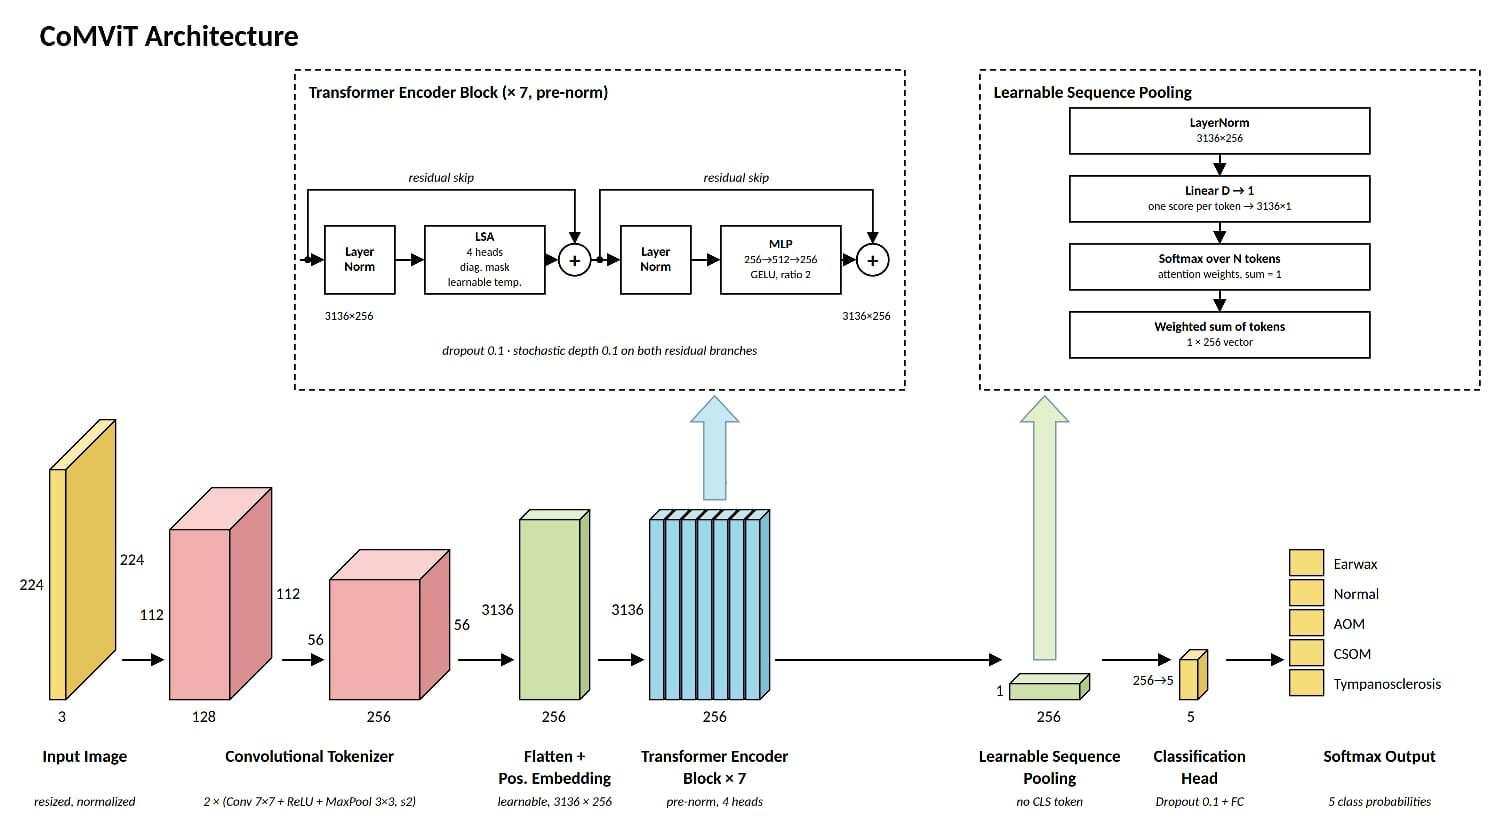
\includegraphics[width=\linewidth, keepaspectratio]{diagrams/architecture.jpeg}
    \caption{Detailed system architecture of the ear disease detection and explainability framework.}
    \label{fig:system_architecture}
\end{figure}

\section{System Workflow and Operational Pipeline}
The operational pipeline progresses across five sequential functional stages shown in Figure~\ref{fig:proposed_pipeline}:
\begin{enumerate}
    \item \textbf{Otoscopic Image Acquisition:} Digital otoscope frame capture, MIME verification, and payload bounding ($\le 10$\,MB).
    \item \textbf{CLAHE Preprocessing:} Contrast enhancement via CLAHE, bilinear resizing to $224 \times 224$, and normalization.
    \item \textbf{CoMViT Feature Extraction:} Local convolutional patch embedding and multi-head self-attention token encoding.
    \item \textbf{5-Class Softmax Classification:} Linear head outputting posterior probabilities across AOM, CSOM, Earwax, Normal, and Tympanosclerosis.
    \item \textbf{Grad-CAM++ Explainability:} Second-order gradient attribution localizing tympanic membrane lesions with Jet colormap overlay.
\end{enumerate}

\begin{figure}[H]
    \centering
    \adjustbox{max width=0.98\linewidth, center}{\documentclass[tikz,border=10pt]{standalone}
\usepackage{tikz}
\usepackage{adjustbox}
\usepackage{fontawesome5}
\usetikzlibrary{arrows.meta,positioning,fit,backgrounds,calc,shadows,shapes.geometric}

% Lavender & Diagnostic Color Palette
\definecolor{lavenderDark}{RGB}{15, 44, 89}
\definecolor{lavenderDeep}{RGB}{10, 28, 58}
\definecolor{lavenderMedium}{RGB}{29, 78, 158}
\definecolor{lavenderLight}{RGB}{240, 246, 255}
\definecolor{lavenderBorder}{RGB}{180, 205, 237}
\definecolor{lavenderAccent}{RGB}{2, 132, 199}
\definecolor{prismNavy}{RGB}{15, 44, 89}
\definecolor{prismBlue}{RGB}{29, 78, 158}
\definecolor{prismTeal}{RGB}{13, 148, 136}
\definecolor{prismMint}{RGB}{236, 253, 245}
\definecolor{prismGold}{RGB}{217, 119, 6}
\definecolor{prismDark}{RGB}{15, 23, 42}
\definecolor{prismLight}{RGB}{248, 250, 252}
\definecolor{cInput}{RGB}{241, 245, 249}
\definecolor{cStem}{RGB}{224, 242, 254}
\definecolor{cStage1}{RGB}{209, 250, 229}
\definecolor{cStage2}{RGB}{254, 243, 199}
\definecolor{cStage3}{RGB}{254, 226, 226}
\definecolor{cStage4}{RGB}{207, 250, 254}
\definecolor{cHead}{RGB}{219, 234, 254}
\definecolor{cOutput}{RGB}{255, 228, 230}

\begin{document}
\begin{tikzpicture}[
  >=Latex,
  stagebox/.style={
    draw=lavenderDark!85,
    rounded corners=7pt,
    minimum height=5.60cm,
    text width=2.72cm,
    align=center,
    inner sep=5pt,
    line width=1.1pt,
    fill=white,
    drop shadow={shadow xshift=1.5pt, shadow yshift=-1.8pt, opacity=0.16}
  },
  pipearrow/.style={
    ->,
    draw=lavenderDark,
    line width=1.8pt,
    arrows={-Latex[length=3.2mm, width=2.4mm]}
  },
  subblk/.style={
    draw=prismNavy!90,
    rounded corners=3.5pt,
    fill=white,
    minimum height=0.88cm,
    text width=0.51cm,
    align=center,
    inner sep=1pt,
    line width=0.85pt,
    drop shadow={shadow xshift=0.6pt, shadow yshift=-0.6pt, opacity=0.10}
  }
]

  % Stage 1: Ingestion
  \node[stagebox, fill=cInput!65] (ingest) {
    \vspace{3pt}
    {\fontsize{16}{18}\selectfont\textcolor{lavenderDark}{\faFileMedical}}\\[4pt]
    {\fontsize{10.5}{12.5}\selectfont\textbf{1. Ingestion}}\\[2pt]
    {\fontsize{7.2}{8.5}\selectfont\textcolor{prismTeal}{\textbf{[Otoscopic Input]}}}\\[5pt]
    \rule{2.4cm}{0.6pt}\\[6pt]
    \begin{minipage}{2.55cm}
      \fontsize{8.0}{9.8}\selectfont
      $\bullet$ Digital Otoscope image\\
      $\bullet$ Eardrum photography\\
      $\bullet$ Merged 5-class set\\
      $\bullet$ Format check (JPG/PNG)\\
      $\bullet$ Resolution validation\\
      $\bullet$ Cerumen / angle check
    \end{minipage}
    \vspace{4pt}
  };

  % Stage 2: Preprocessing
  \node[stagebox, fill=cStage1!60, right=0.22cm of ingest] (preprocess) {
    \vspace{3pt}
    {\fontsize{16}{18}\selectfont\textcolor{prismTeal}{\faSlidersH}}\\[4pt]
    {\fontsize{10.5}{12.5}\selectfont\textbf{2. Preprocessing}}\\[2pt]
    {\fontsize{7.2}{8.5}\selectfont\textcolor{prismTeal}{\textbf{[CLAHE \& MixUp]}}}\\[5pt]
    \rule{2.4cm}{0.6pt}\\[6pt]
    \begin{minipage}{2.55cm}
      \fontsize{8.0}{9.8}\selectfont
      $\bullet$ CLAHE equalization\\
      $\bullet$ Resize to $224 \times 224$\\
      $\bullet$ Channel normalization\\
      $\bullet$ Online data augment\\
      $\bullet$ Controlled MixUp\\
      $\bullet$ Curriculum weighting
    \end{minipage}
    \vspace{4pt}
  };

  % Stage 3: CoMViT
  \node[stagebox, text width=2.82cm, fill=cStem!60, draw=lavenderDark!95, line width=1.3pt, right=0.20cm of preprocess] (comvit) {
    \vspace{3pt}
    {\fontsize{16}{18}\selectfont\textcolor{lavenderDark}{\faBrain}}\\[4pt]
    {\fontsize{10.5}{12.5}\selectfont\textbf{3. CoMViT Model}}\\[2pt]
    {\fontsize{7.2}{8.5}\selectfont\textcolor{lavenderDark}{\textbf{[Local \& Global ViT]}}}\\[4pt]
    \rule{2.5cm}{0.6pt}\\[4pt]
    \begin{tikzpicture}[baseline=-0.3ex, node distance=0.10cm]
      \node[subblk, fill=cStem!55] (b1) {{\fontsize{8.0}{9}\selectfont\textbf{Conv}}\\[1pt]{\fontsize{5.2}{6}\selectfont\color{prismDark!75}Stem}};
      \node[subblk, fill=cStage4!55, right=0.10cm of b1] (b2) {{\fontsize{8.0}{9}\selectfont\textbf{MHSA}}\\[1pt]{\fontsize{5.2}{6}\selectfont\color{prismDark!75}Attn}};
      \node[subblk, fill=cStage2!55, right=0.10cm of b2] (b3) {{\fontsize{8.0}{9}\selectfont\textbf{Trans}}\\[1pt]{\fontsize{5.2}{6}\selectfont\color{prismDark!75}Blk}};
      \node[subblk, fill=cStage3!55, right=0.10cm of b3] (b4) {{\fontsize{8.0}{9}\selectfont\textbf{MLP}}\\[1pt]{\fontsize{5.2}{6}\selectfont\color{prismDark!75}Head}};
      \draw[->, draw=prismNavy, line width=0.85pt, arrows={-Latex[length=1.6mm, width=1.2mm]}, shorten >=0.5pt, shorten <=0.5pt] (b1) -- (b2);
      \draw[->, draw=prismNavy, line width=0.85pt, arrows={-Latex[length=1.6mm, width=1.2mm]}, shorten >=0.5pt, shorten <=0.5pt] (b2) -- (b3);
      \draw[->, draw=prismNavy, line width=0.85pt, arrows={-Latex[length=1.6mm, width=1.2mm]}, shorten >=0.5pt, shorten <=0.5pt] (b3) -- (b4);
    \end{tikzpicture}\\[5pt]
    \begin{minipage}{2.65cm}
      \fontsize{8.0}{9.8}\selectfont
      $\bullet$ Hybrid inductive bias\\
      $\bullet$ Multi-head attention\\
      $\bullet$ Local patch features\\
      $\bullet$ Global eardrum context
    \end{minipage}
    \vspace{4pt}
  };

  % Stage 4: Classification
  \node[stagebox, fill=cHead!60, right=0.22cm of comvit] (classify) {
    \vspace{3pt}
    {\fontsize{16}{18}\selectfont\textcolor{lavenderDark}{\faChartPie}}\\[4pt]
    {\fontsize{10.5}{12.5}\selectfont\textbf{4. Classify}}\\[2pt]
    {\fontsize{7.2}{8.5}\selectfont\textcolor{lavenderDark}{\textbf{[5-Class Softmax]}}}\\[5pt]
    \rule{2.4cm}{0.6pt}\\[6pt]
    \begin{minipage}{2.55cm}
      \fontsize{7.5}{9.2}\selectfont
      $\bullet$ Softmax vector $\hat{\mathbf{y}} \in \mathbb{R}^5$:\\[2pt]
      \phantom{$\bullet$}\,$\circ$ \textbf{AOM}\\
      \phantom{$\bullet$}\,$\circ$ \textbf{CSOM}\\
      \phantom{$\bullet$}\,$\circ$ \textbf{Earwax}\\
      \phantom{$\bullet$}\,$\circ$ \textbf{Normal}\\
      \phantom{$\bullet$}\,$\circ$ \textbf{Tympanosclerosis}
    \end{minipage}
    \vspace{4pt}
  };

  % Stage 5: Explainability
  \node[stagebox, fill=cStage2!65, draw=prismGold!95!black, line width=1.2pt, right=0.22cm of classify] (explain) {
    \vspace{3pt}
    {\fontsize{16}{18}\selectfont\textcolor{prismGold!95!black}{\faFire}}\\[4pt]
    {\fontsize{10.5}{12.5}\selectfont\textbf{5. Explain}}\\[2pt]
    {\fontsize{7.2}{8.5}\selectfont\textcolor{prismGold!95!black}{\textbf{[Grad-CAM++]}}}\\[5pt]
    \rule{2.4cm}{0.6pt}\\[6pt]
    \begin{minipage}{2.55cm}
      \fontsize{8.0}{9.8}\selectfont
      $\bullet$ 2nd-order gradients\\
      $\bullet$ TM region attribution\\
      $\bullet$ Localizes perforation /\\
      \phantom{$\bullet$}\,bulging / plaques\\
      $\bullet$ Alpha-blended overlay\\
      $\bullet$ Clinical verification
    \end{minipage}
    \vspace{4pt}
  };

  % Connecting Arrows
  \draw[pipearrow] (ingest.east) -- (preprocess.west);
  \draw[pipearrow] (preprocess.east) -- (comvit.west);
  \draw[pipearrow] (comvit.east) -- (classify.west);
  \draw[pipearrow] (classify.east) -- (explain.west);

\end{tikzpicture}
\end{document}
}
    \caption{Proposed operational pipeline of the deep learning ear disease detection and explainability framework.}
    \label{fig:proposed_pipeline}
\end{figure}

Figure~\ref{fig:layered_workflow} maps the complete lifecycle and feedback pathways connecting acquisition, validation, CoMViT feature learning, Grad-CAM++ attribution, classification, and screening delivery.

\begin{figure}[H]
    \centering
    \adjustbox{max width=0.98\linewidth, max height=0.72\textheight, keepaspectratio, center}{\documentclass[tikz,border=10pt]{standalone}
\usepackage{tikz}
\usepackage{fontawesome5}
\usetikzlibrary{arrows.meta,positioning,fit,backgrounds,calc,shadows,shapes.geometric}

% Color definitions
\definecolor{lavenderDark}{RGB}{15, 44, 89}
\definecolor{lavenderDeep}{RGB}{10, 28, 58}
\definecolor{lavenderMedium}{RGB}{29, 78, 158}
\definecolor{lavenderLight}{RGB}{240, 246, 255}
\definecolor{lavenderBorder}{RGB}{180, 205, 237}
\definecolor{lavenderAccent}{RGB}{2, 132, 199}
\definecolor{prismNavy}{RGB}{15, 44, 89}
\definecolor{prismBlue}{RGB}{29, 78, 158}
\definecolor{prismTeal}{RGB}{13, 148, 136}
\definecolor{prismMint}{RGB}{236, 253, 245}
\definecolor{prismGold}{RGB}{217, 119, 6}
\definecolor{prismDark}{RGB}{15, 23, 42}
\definecolor{prismLight}{RGB}{248, 250, 252}
\definecolor{prismIndigo}{RGB}{30, 58, 138}
\definecolor{prismSlate}{RGB}{100, 116, 139}
\definecolor{statusFail}{RGB}{220, 38, 38}
\definecolor{cInput}{RGB}{241, 245, 249}
\definecolor{cStem}{RGB}{224, 242, 254}
\definecolor{cStage1}{RGB}{209, 250, 229}
\definecolor{cStage2}{RGB}{254, 243, 199}
\definecolor{cStage3}{RGB}{254, 226, 226}
\definecolor{cStage4}{RGB}{207, 250, 254}
\definecolor{cHead}{RGB}{219, 234, 254}
\definecolor{cOutput}{RGB}{255, 228, 230}
\definecolor{cDeliverable}{RGB}{204, 251, 241}

\begin{document}
% Complete Layered System Workflow for Ear Disease Detection
\begin{tikzpicture}[
    x=1cm, y=1cm,
    font=\sffamily,
    stepbox/.style={
        rectangle, draw=lavenderDark!85, line width=0.95pt, fill=white,
        rounded corners=4pt, inner sep=5pt, align=center,
        drop shadow={shadow xshift=1pt, shadow yshift=-1pt, opacity=0.15}
    },
    flowarr/.style={
        -{Stealth[scale=1.05]}, line width=1.25pt, draw=lavenderDark!90
    },
    dashloop/.style={
        -{Stealth[scale=1.0]}, line width=1.15pt, dashed, draw=prismGold!95!black
    }
]

    % Step 1: Otoscopic Acquisition
    \node [stepbox, fill=cInput, text width=2.65cm] (b1) at (-5.75, 0) {
        \textbf{\fontsize{9.6}{11.5}\selectfont\color{lavenderDark}1. Otoscopic Acquisition}\\[0.3em]
        \fontsize{8.0}{9.5}\selectfont
        $\bullet$ Digital otoscope input\\
        $\bullet$ Bedside video endoscope\\
        $\bullet$ Multipart streaming
    };

    % Step 2: Validation & CLAHE Preprocessing
    \node [stepbox, fill=cStage1, text width=2.65cm] (b2) at (-2.65, 0) {
        \textbf{\fontsize{9.6}{11.5}\selectfont\color{lavenderDark}2. CLAHE \& Validation}\\[0.3em]
        \fontsize{8.0}{9.5}\selectfont
        $\bullet$ MIME \& cerumen check\\
        $\bullet$ CLAHE enhancement\\
        $\bullet$ Resize to $224 \times 224$
    };

    % Step 3: CoMViT Backbone
    \node [stepbox, fill=cStem, text width=3.85cm] (b3) at (1.45, 1.80) {
        \textbf{\fontsize{9.6}{11.5}\selectfont\color{lavenderDark}3. CoMViT Backbone}\\[0.28em]
        \fontsize{7.8}{9.4}\selectfont
        {\color{prismIndigo}\faLayerGroup}\; \textbf{Conv Stem:} Local patch embedding\\[0.15em]
        {\color{prismBlue}\faProjectDiagram}\; \textbf{Multi-Head Attention:} Global TM\\[0.15em]
        {\color{prismTeal}\faCompress}\; \textbf{Curriculum Learning:} Adaptive loss\\[0.15em]
        {\color{purple!75!black}\faNetworkWired}\; \textbf{Token Latent:} Rich representation
    };

    % Step 4: Grad-CAM++ Engine
    \node [stepbox, fill=cStage2, text width=3.85cm] (b4) at (1.45, -1.80) {
        \textbf{\fontsize{9.6}{11.5}\selectfont\color{lavenderDark}4. Grad-CAM++ Engine}\\[0.28em]
        \fontsize{7.8}{9.4}\selectfont
        {\color{prismGold!90!black}\faLink}\; \textbf{Hook:} Target transformer block\\[0.15em]
        {\color{prismBlue}\faCalculator}\; \textbf{2nd-Order Gradients:} $\alpha_{ijk}^c$ pooling\\[0.15em]
        {\color{prismTeal}\faEye}\; \textbf{Positive Attribution:} TM localization\\[0.15em]
        {\color{red!70!black}\faPalette}\; \textbf{Color Overlay:} Lesion saliency map
    };

    % Step 5: Softmax Classification across 5 Classes
    \node [stepbox, fill=cHead, text width=2.65cm] (b5) at (5.55, 0) {
        \textbf{\fontsize{9.6}{11.5}\selectfont\color{lavenderDark}5. 5-Class Scoring}\\[0.3em]
        \fontsize{7.8}{9.2}\selectfont
        $\bullet$ Linear head $\to 5$ classes\\
        $\bullet$ Softmax probability\\
        $\bullet$ AOM, CSOM, Earwax,\\
        \phantom{$\bullet$}\,Normal, Tympanosclerosis
    };

    % Step 6: Diagnostic Delivery & Triage
    \node [stepbox, fill=cDeliverable!80, text width=3.85cm] (b6) at (9.65, 0) {
        \textbf{\fontsize{9.6}{11.5}\selectfont\color{lavenderDark}6. Clinical Decision Support}\\[0.28em]
        \fontsize{7.8}{9.4}\selectfont
        {\color{prismNavy}\faDesktop}\; \textbf{Web Portal:} Diagnostic visualization\\[0.15em]
        {\color{lavenderDark}\faMobile}\; \textbf{Mobile App:} Bedside otoscopy scan\\[0.15em]
        {\color{prismTeal}\faClock}\; \textbf{FastAPI Serving:} Sub-50\,ms latency\\[0.15em]
        {\color{red!75!black}\faShieldVirus}\; \textbf{Clinical Guidance:} ENT verification
    };

    % 1. Connect Step 1 -> Step 2
    \draw [flowarr] (b1) -- (b2);

    % 2. Clean Split from Validation into CoMViT and Grad-CAM++
    \coordinate (split1) at ($(b2.east)!0.5!(b3.west |- b2.east)$);
    \draw [line width=1.25pt, draw=lavenderDark!90] (b2.east) -- (split1);
    \draw [flowarr] (split1) |- (b3.west);
    \draw [flowarr] (split1) |- (b4.west);

    % 3. Bidirectional interactive link between Features and Grad-CAM++ Hook
    \draw [{Stealth[scale=1.05]}-{Stealth[scale=1.05]}, line width=1.25pt, draw=prismTeal] (b3.south) -- (b4.north);

    % 4. Convergence into Classification
    \coordinate (join1) at ($(b3.east |- b5.west)!0.5!(b5.west)$);
    \draw [line width=1.25pt, draw=lavenderDark!90] (b3.east) -| (join1);
    \draw [line width=1.25pt, draw=lavenderDark!90] (b4.east) -| (join1);
    \draw [flowarr] (join1) -- (b5.west);

    % 5. Connect Step 5 -> Step 6
    \draw [flowarr] (b5) -- (b6);

    % 6. Quality and Re-acquisition Feedback Loop
    \draw [dashloop] (b5.north) -- (b5.north |- 0, 3.45) 
        -- node[above=2.5pt, font=\fontsize{8.2}{9.8}\selectfont\bfseries\color{prismGold!95!black}]{Otoscopic Quality Audit \& Visibility Re-Check} (b2.north |- 0, 3.45) 
        -- (b2.north);

\end{tikzpicture}
\end{document}
}
    \caption{Layered system workflow and 6-stage execution lifecycle across acquisition, validation, CoMViT backbone, Grad-CAM++ engine, scoring, and delivery.}
    \label{fig:layered_workflow}
\end{figure}

Figure~\ref{fig:end_to_end_flow} illustrates the end-to-end data flow transitioning from the raw otoscopic input bar to the verified clinical screening output.

\begin{figure}[H]
    \centering
    \adjustbox{max width=0.98\linewidth, max height=0.72\textheight, keepaspectratio, center}{\documentclass[tikz,border=8pt]{standalone}
\usepackage{tikz}
\usepackage{fontawesome5}
\usepackage{amsmath,amssymb}
\usetikzlibrary{arrows.meta,positioning,fit,backgrounds,calc,shadows,shapes.geometric}

% Lavender Color Palette
\definecolor{lavenderDark}{RGB}{15, 44, 89}
\definecolor{lavenderDeep}{RGB}{10, 28, 58}
\definecolor{lavenderMedium}{RGB}{29, 78, 158}
\definecolor{lavenderLight}{RGB}{240, 246, 255}
\definecolor{lavenderBorder}{RGB}{180, 205, 237}
\definecolor{lavenderAccent}{RGB}{2, 132, 199}
\definecolor{prismNavy}{RGB}{15, 44, 89}
\definecolor{prismBlue}{RGB}{29, 78, 158}
\definecolor{prismTeal}{RGB}{13, 148, 136}
\definecolor{prismMint}{RGB}{236, 253, 245}
\definecolor{prismGold}{RGB}{217, 119, 6}
\definecolor{prismDark}{RGB}{15, 23, 42}
\definecolor{prismLight}{RGB}{248, 250, 252}

\begin{document}
% End-to-End System Flow for Deep Learning Ear Disease Detection
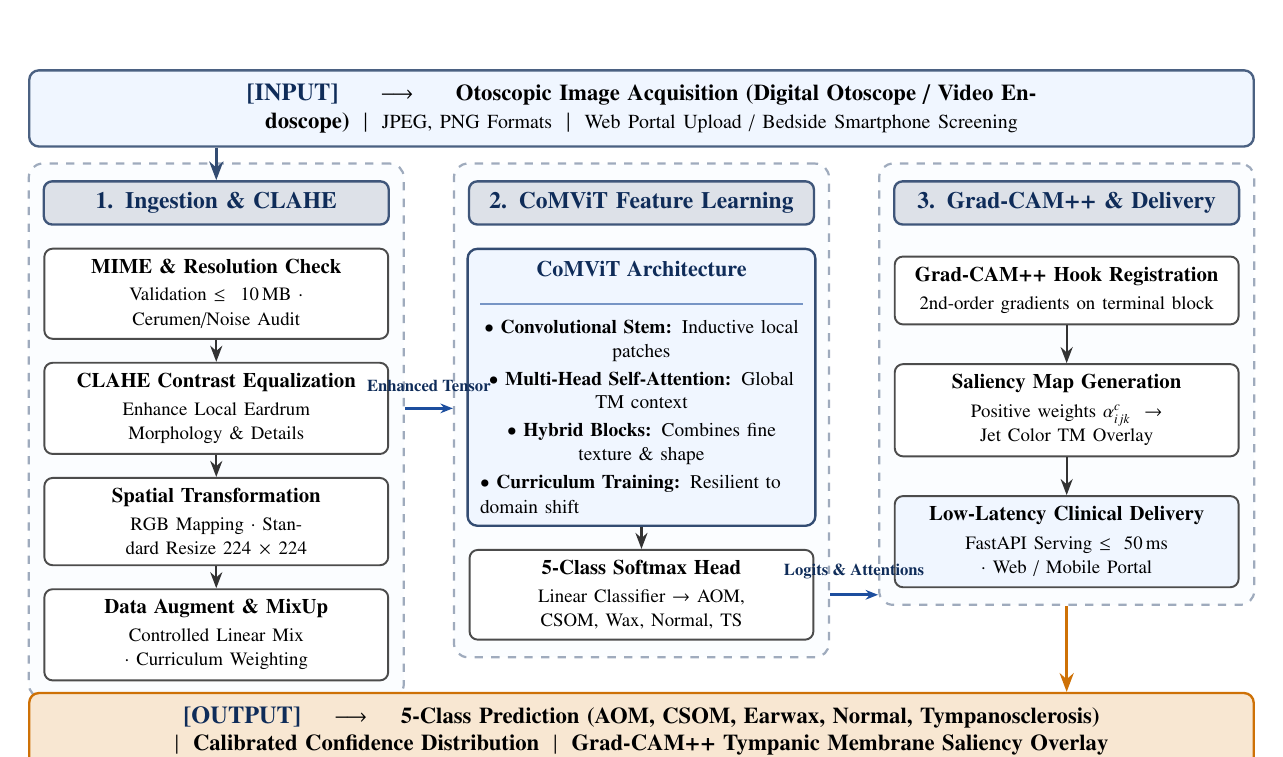
\begin{tikzpicture}[
    x=1cm, y=1cm,
    font=\sffamily,
    inout/.style={
        rectangle, rounded corners=3.5pt, line width=0.85pt,
        inner sep=5pt, align=center,
        font=\fontsize{8.2}{9.8}\selectfont
    },
    hdrbox/.style={
        rectangle, draw=lavenderDark!80, line width=0.85pt, fill=lavenderDark!14,
        rounded corners=3pt, inner sep=4pt, align=center,
        text width=4.10cm,
        font=\fontsize{8.5}{10.2}\selectfont\bfseries\color{lavenderDark}
    },
    stepbox/.style={
        rectangle, draw=black!70, line width=0.7pt, fill=white,
        rounded corners=3pt, inner sep=3.8pt, align=center,
        text width=4.10cm,
        font=\fontsize{7.5}{8.8}\selectfont
    },
    enginebox/.style={
        rectangle, draw=lavenderDark!85, line width=0.85pt, fill=lavenderLight,
        rounded corners=3.5pt, inner sep=4.5pt, align=left,
        text width=4.10cm,
        font=\fontsize{7.2}{8.8}\selectfont
    },
    stagebox/.style={
        rectangle, draw=lavenderDark!40, dashed, rounded corners=5pt, line width=0.8pt,
        fill=lavenderLight!25, inner xsep=5pt, inner ysep=6pt
    },
    flowarr/.style={
        -{Stealth[scale=0.85]}, line width=0.85pt, draw=black!80
    },
    transarr/.style={
        -{Stealth[length=4.5pt, width=3.5pt]}, line width=1.1pt, draw=lavenderMedium
    }
]

    % 1. TOP: INPUT BAR
    \node [inout, fill=lavenderLight, draw=lavenderDark!75, text width=15.2cm] (input_node) at (0, 3.40) {
        \textbf{\fontsize{8.8}{10.4}\selectfont\color{lavenderDark}[INPUT]} $\;\longrightarrow\;$
        \textbf{Otoscopic Image Acquisition (Digital Otoscope / Video Endoscope)}\; $\vert$\;
        {\fontsize{7.2}{8.5}\selectfont JPEG, PNG Formats}\; $\vert$\;
        {\fontsize{7.2}{8.5}\selectfont Web Portal Upload / Bedside Smartphone Screening}
    };

    % 2. MIDDLE: 3-STAGE HORIZONTAL PIPELINE

    % --- STAGE 1: INGESTION & PREPROCESSING ---
    \node [hdrbox] (h1) at (-5.40, 2.20) {1. Ingestion \& CLAHE};
    \node [stepbox, below=0.28cm of h1] (s1_1) {
        \textbf{MIME \& Resolution Check}\\[0.15em]
        {\fontsize{6.8}{8.0}\selectfont Validation $\le 10$\,MB $\cdot$ Cerumen/Noise Audit}
    };
    \node [stepbox, below=0.28cm of s1_1] (s1_2) {
        \textbf{CLAHE Contrast Equalization}\\[0.15em]
        {\fontsize{6.8}{8.0}\selectfont Enhance Local Eardrum Morphology \& Details}
    };
    \node [stepbox, below=0.28cm of s1_2] (s1_3) {
        \textbf{Spatial Transformation}\\[0.15em]
        {\fontsize{6.8}{8.0}\selectfont RGB Mapping $\cdot$ Standard Resize $224\times 224$}
    };
    \node [stepbox, below=0.28cm of s1_3] (s1_4) {
        \textbf{Data Augment \& MixUp}\\[0.15em]
        {\fontsize{6.8}{8.0}\selectfont Controlled Linear Mix $\cdot$ Curriculum Weighting}
    };

    \draw [flowarr] (s1_1) -- (s1_2);
    \draw [flowarr] (s1_2) -- (s1_3);
    \draw [flowarr] (s1_3) -- (s1_4);

    \begin{scope}[on background layer]
    \node [stagebox, fit=(h1) (s1_4)] (stage1) {};
    \end{scope}

    % --- STAGE 2: COMVIT INFERENCE ---
    \node [hdrbox] (h2) at (0, 2.20) {2. CoMViT Feature Learning};
    \node [enginebox, below=0.28cm of h2] (s2_1) {
        \centering\textbf{\fontsize{8.0}{9.5}\selectfont\color{lavenderDark}CoMViT Architecture}\\[0.2em]
        {\color{lavenderMedium!60}\rule{\linewidth}{0.5pt}}\\[0.28em]
        {\fontsize{7.0}{8.5}\selectfont
        $\bullet$ \textbf{Convolutional Stem:} Inductive local patches\\[0.22em]
        $\bullet$ \textbf{Multi-Head Self-Attention:} Global TM context\\[0.22em]
        $\bullet$ \textbf{Hybrid Blocks:} Combines fine texture \& shape\\[0.22em]
        $\bullet$ \textbf{Curriculum Training:} Resilient to domain shift}
    };

    \node [stepbox, below=0.28cm of s2_1] (s2_2) {
        \textbf{5-Class Softmax Head}\\[0.15em]
        {\fontsize{6.8}{8.0}\selectfont Linear Classifier $\to$ AOM, CSOM, Wax, Normal, TS}
    };

    \draw [flowarr] (s2_1) -- (s2_2);

    \begin{scope}[on background layer]
    \node [stagebox, fit=(h2) (s2_2)] (stage2) {};
    \end{scope}

    % --- STAGE 3: GRAD-CAM++ & DELIVERY ---
    \node [hdrbox] (h3) at (5.40, 2.20) {3. Grad-CAM++ \& Delivery};
    \node [stepbox, below=0.38cm of h3] (s3_1) {
        \textbf{Grad-CAM++ Hook Registration}\\[0.2em]
        {\fontsize{6.8}{8.0}\selectfont 2nd-order gradients on terminal block}
    };
    \node [stepbox, below=0.48cm of s3_1] (s3_2) {
        \textbf{Saliency Map Generation}\\[0.2em]
        {\fontsize{6.8}{8.0}\selectfont Positive weights $\alpha_{ijk}^c \to$ Jet Color TM Overlay}
    };
    \node [stepbox, below=0.48cm of s3_2, fill=lavenderLight] (s3_3) {
        \textbf{Low-Latency Clinical Delivery}\\[0.2em]
        {\fontsize{6.8}{8.0}\selectfont FastAPI Serving $\le 50$\,ms $\cdot$ Web / Mobile Portal}
    };

    \draw [flowarr] (s3_1) -- (s3_2);
    \draw [flowarr] (s3_2) -- (s3_3);

    \begin{scope}[on background layer]
    \node [stagebox, fit=(h3) (s3_3)] (stage3) {};
    \end{scope}

    % Transition arrows between stages
    \draw [transarr] (stage1.east |- s1_2) -- 
        node[above=2pt, font=\fontsize{6.0}{7.0}\selectfont\bfseries\color{lavenderDark}]{Enhanced Tensor} (stage2.west |- s1_2);

    \draw [transarr] (stage2.east |- s2_2) -- 
        node[above=2pt, font=\fontsize{6.0}{7.0}\selectfont\bfseries\color{lavenderDark}]{Logits \& Attentions} (stage3.west |- s2_2);

    \draw [flowarr, line width=1.1pt, draw=lavenderDark!85] (input_node.south -| h1.north) -- (h1.north);

    % 3. BOTTOM: OUTPUT BAR
    \node [inout, fill=prismGold!18, draw=prismGold!95!black, text width=15.2cm, below=0.50cm of $(stage1.south)!0.5!(stage3.south)$] (output_node) {
        \textbf{\fontsize{8.8}{10.4}\selectfont\color{lavenderDark}[OUTPUT]} $\;\longrightarrow\;$
        \textbf{5-Class Prediction (AOM, CSOM, Earwax, Normal, Tympanosclerosis)}\; $\vert$\;
        \textbf{Calibrated Confidence Distribution}\; $\vert$\;
        \textbf{Grad-CAM++ Tympanic Membrane Saliency Overlay}
    };

    \draw [flowarr, line width=1.1pt, draw=prismGold!95!black] (stage3.south -| h3.south) -- (output_node.north -| h3.south);

\end{tikzpicture}
\end{document}
}
    \caption{Overall end-to-end system flow architecture from raw otoscopic image ingestion through CLAHE, CoMViT inference, and Grad-CAM++ saliency delivery.}
    \label{fig:end_to_end_flow}
\end{figure}

\section{System Flowchart and Algorithms}

\subsection{System Flowchart}
Figure~\ref{fig:multiagent_flowchart} maps the complete execution logic, preprocessing steps, convolutional tokenization, transformer attention sequence, classification, and Grad-CAM explainability workflow executing during clinical inference requests.

\begin{figure}[H]
    \centering
    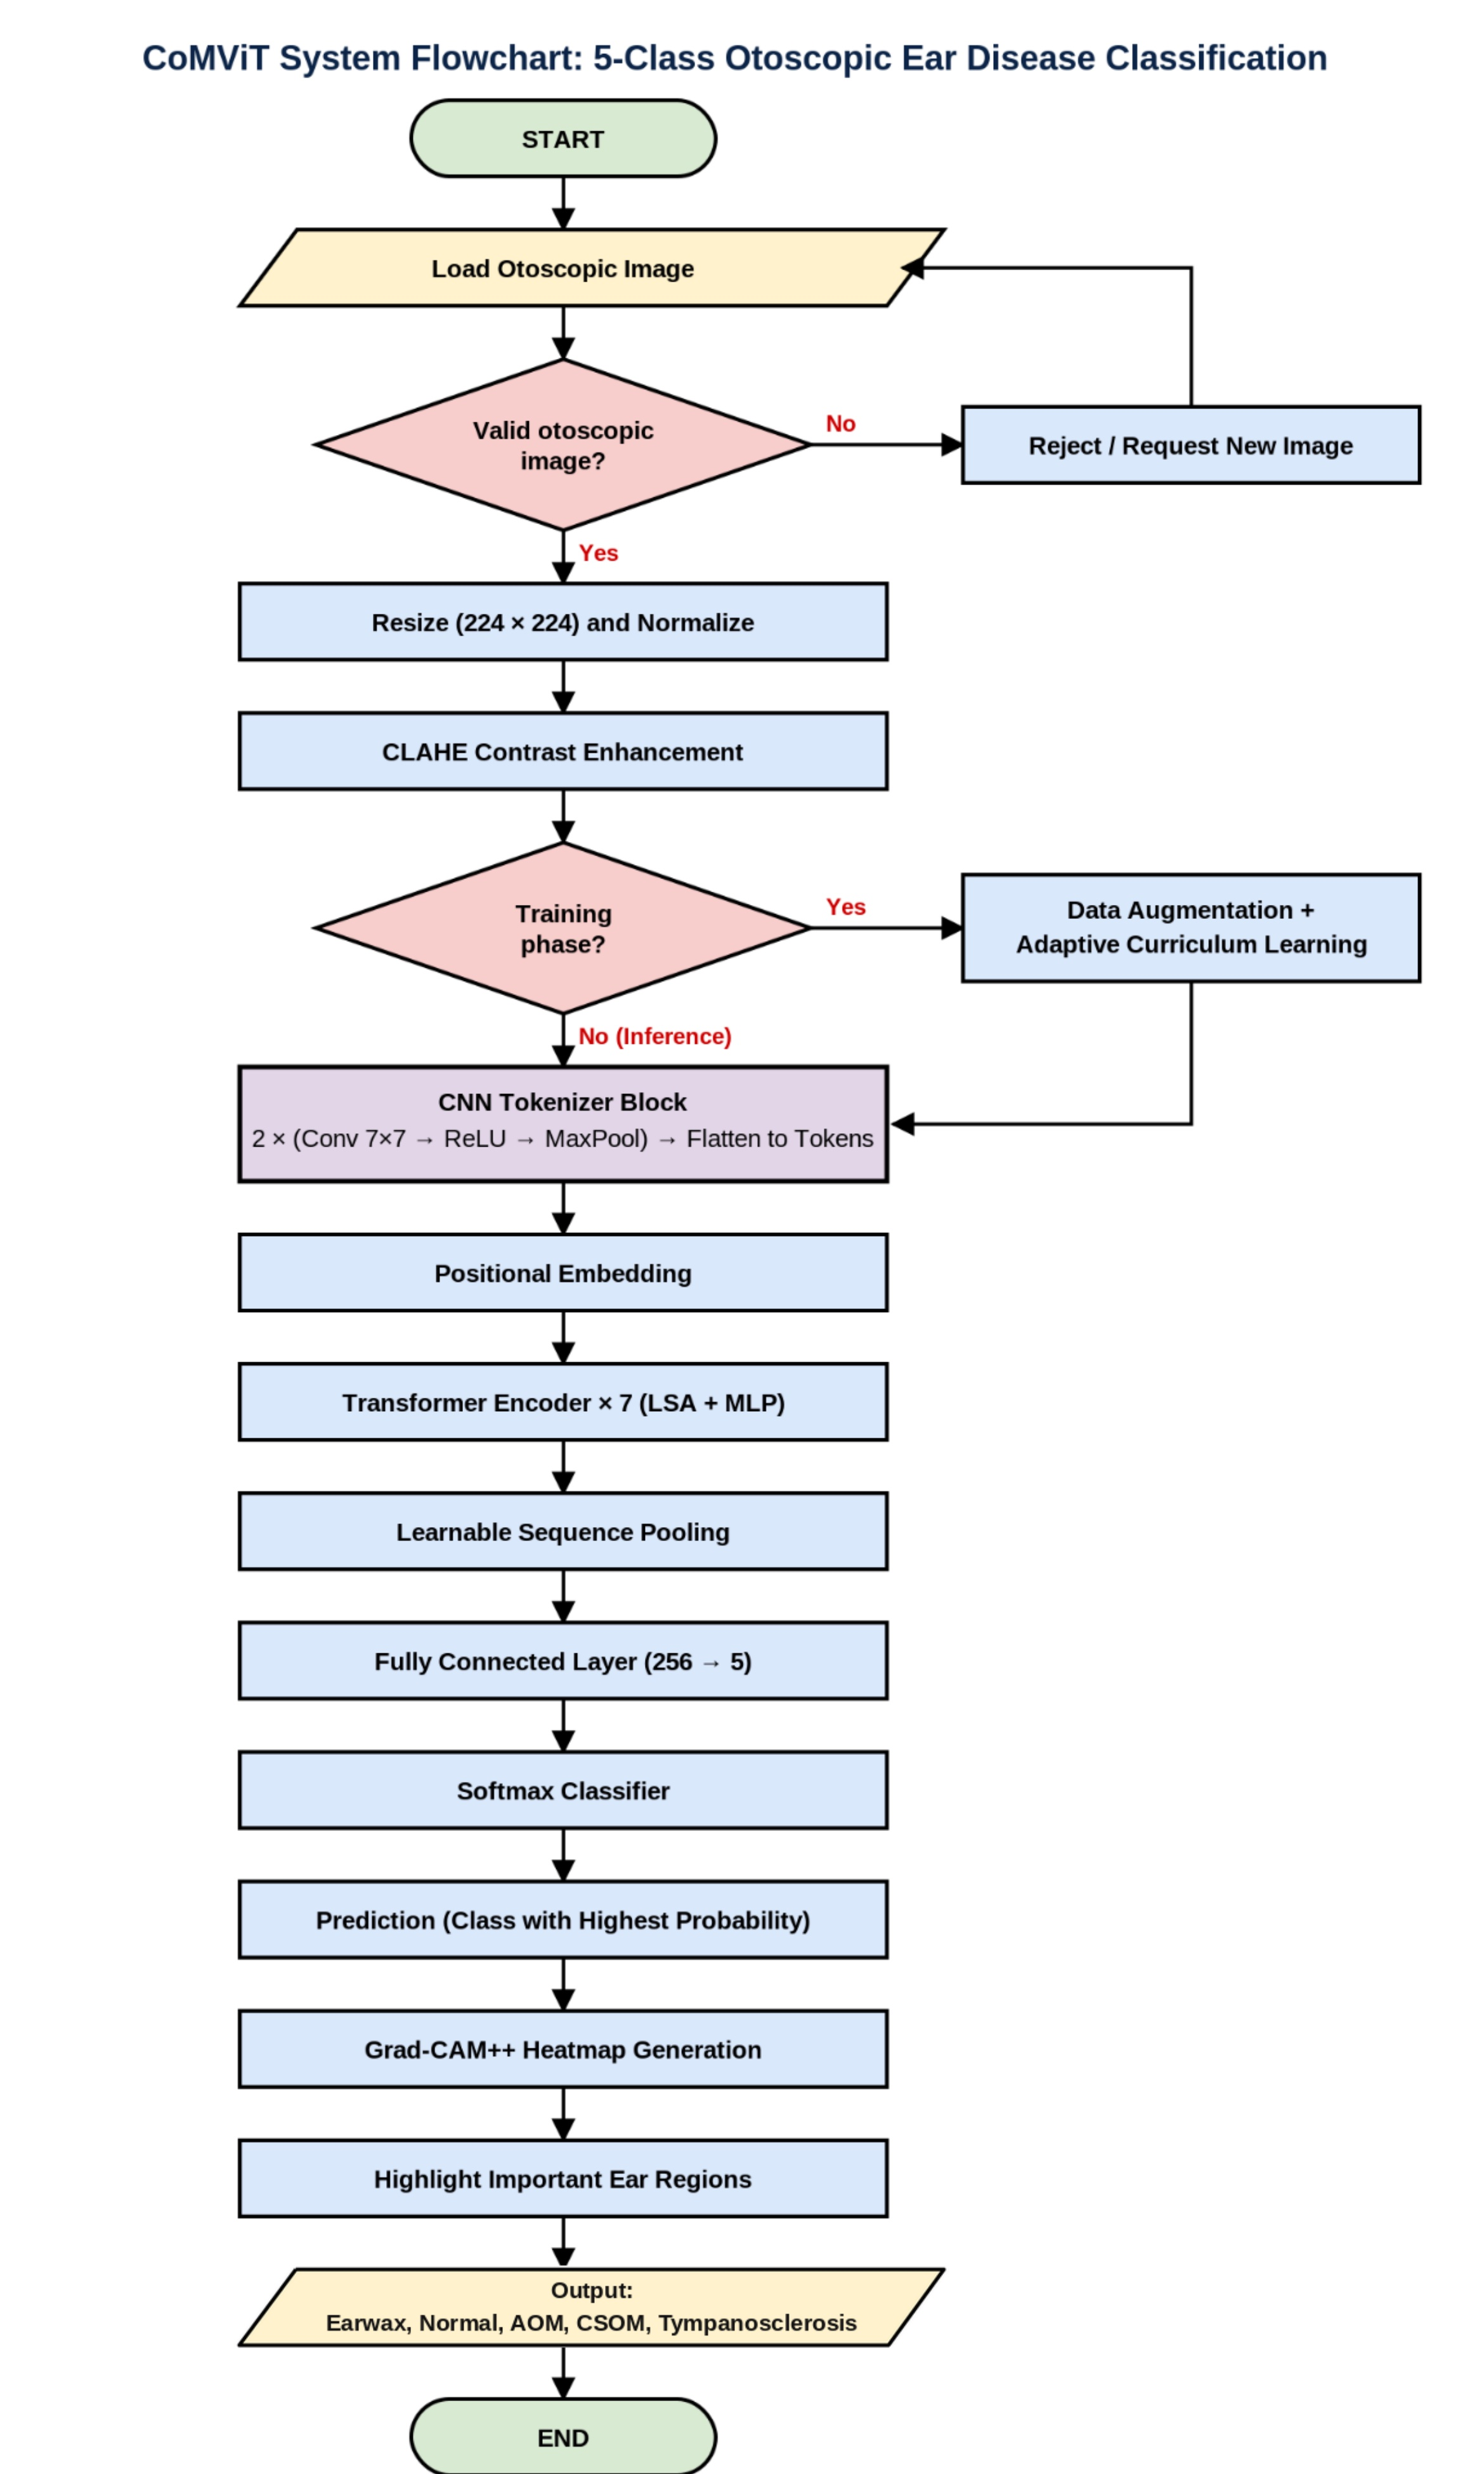
\includegraphics[width=0.92\linewidth, height=0.83\textheight, keepaspectratio]{diagrams/flowchart.jpeg}
    \caption{System flowchart detailing otoscopic image ingestion, preprocessing, convolutional tokenization, Locality Self-Attention transformer encoding, classification, and Grad-CAM explanation generation.}
    \label{fig:multiagent_flowchart}
\end{figure}

\subsection{System Algorithm}
The complete operational algorithm of the ear disease classification and explainability framework is formalized below across six sequential stages:

\subsubsection*{Step 1: Data Loading and Preprocessing}
\begin{enumerate}
  \item[\textbf{1.1}] Import the otoscopic dataset encompassing the five diagnostic categories: Earwax, Normal, Acute Otitis Media (AOM), Chronic Suppurative Otitis Media (CSOM), and Tympanosclerosis.
  \item[\textbf{1.2}] Split the dataset into training, validation, and testing sets.
  \item[\textbf{1.3}] Resize every image to $224 \times 224$ pixels and normalize pixel values to $[0, 1]$:
    \begin{equation}
      x' = \frac{x}{255}
    \end{equation}
  \item[\textbf{1.4}] Apply data augmentation (rotation, horizontal and vertical flipping, brightness adjustments, and zooming) to the training set (optional).
\end{enumerate}

\subsubsection*{Step 2: Convolutional Tokenization}
\begin{enumerate}
  \item[\textbf{2.1}] Input the preprocessed image ($224 \times 224 \times 3$) to the tokenizer configured with two convolutional stages.
  \item[\textbf{2.2}] Apply $\text{Conv2D}\,(7 \times 7)$ filters to extract inductive local features such as edges and textures.
  \item[\textbf{2.3}] Apply Rectified Linear Unit activation, $f(x) = \max(0, x)$, and max pooling to reduce the spatial size to $56 \times 56 \times 256$.
  \item[\textbf{2.4}] Flatten the feature map into $N = 3136$ tokens of dimension $D = 256$ and add learnable positional embeddings.
\end{enumerate}

\subsubsection*{Step 3: Transformer Encoder (Repeated 7 Times)}
\begin{enumerate}
  \item[\textbf{3.1}] Apply Layer Normalization ($\mathrm{LN}$) to the token sequence $\mathbf{Z} \in \mathbb{R}^{N \times D}$.
  \item[\textbf{3.2}] Apply Locality Self-Attention (LSA) with a diagonal mask and a learnable temperature $\tau$:
    \begin{equation}
      \mathrm{Attention}(\mathbf{Q}, \mathbf{K}, \mathbf{V}) = \mathrm{softmax}\left( \frac{\mathbf{Q}\mathbf{K}^T}{\tau} + \mathbf{M} \right) \mathbf{V}, \quad M_{ii} = -\infty
    \end{equation}
  \item[\textbf{3.3}] Add the residual connection following the attention mechanism:
    \begin{equation}
      \mathbf{Z}' = \mathbf{Z} + \mathrm{LSA}\big( \mathrm{LN}(\mathbf{Z}) \big)
    \end{equation}
  \item[\textbf{3.4}] Apply Layer Normalization, feed into the Multi-Layer Perceptron (MLP feed-forward network with GELU activation), and add the residual connection:
    \begin{equation}
      \mathbf{Z}'' = \mathbf{Z}' + \mathrm{MLP}\big( \mathrm{LN}(\mathbf{Z}') \big)
    \end{equation}
\end{enumerate}

\subsubsection*{Step 4: Sequence Pooling, Classification and Loss Computation}
\begin{enumerate}
  \item[\textbf{4.1}] Apply learnable sequence pooling (without requiring a dedicated [CLS] token) to generate a weighted summary representation across all tokens:
    \begin{equation}
      \mathbf{a} = \mathrm{softmax}\Big( \mathrm{Linear}\big( \mathrm{LN}(\mathbf{Z}) \big) \Big), \quad \mathbf{z} = \mathbf{a}^T \mathbf{Z} \quad (1 \times 256)
    \end{equation}
  \item[\textbf{4.2}] Apply Dropout regularization, followed by a fully-connected projection classification layer ($256 \to 5$).
  \item[\textbf{4.3}] Apply the Softmax activation function to calculate the posterior probability for each of the 5 classes:
    \begin{equation}
      P_i = \frac{\exp(z_i)}{\sum_{j=1}^5 \exp(z_j)}, \quad i \in \{1, \dots, 5\}
    \end{equation}
  \item[\textbf{4.4}] Compute the categorical cross-entropy loss, backpropagate error gradients, and update network parameters using the Adam optimizer:
    \begin{equation}
      \mathcal{L} = -\sum_{i=1}^5 y_i \log(P_i)
    \end{equation}
\end{enumerate}

\subsubsection*{Step 5: Model Evaluation}
\begin{enumerate}
  \item[\textbf{5.1}] Evaluate the trained model on the unseen validation and test partitions.
  \item[\textbf{5.2}] Calculate Accuracy, Precision, Recall, and F1-score (per diagnostic class, followed by macro-averaging across all five classes):
    \begin{align}
      \mathrm{Accuracy}  &= \frac{\mathrm{TP} + \mathrm{TN}}{\mathrm{TP} + \mathrm{TN} + \mathrm{FP} + \mathrm{FN}} \\
      \mathrm{Precision} &= \frac{\mathrm{TP}}{\mathrm{TP} + \mathrm{FP}} \\
      \mathrm{Recall}    &= \frac{\mathrm{TP}}{\mathrm{TP} + \mathrm{FN}} \\
      \text{F1-score}    &= \frac{2 \times (\mathrm{Precision} \times \mathrm{Recall})}{\mathrm{Precision} + \mathrm{Recall}}
    \end{align}
\end{enumerate}

\subsubsection*{Step 6: Generate a Grad-CAM Explanation}
\begin{enumerate}
  \item[\textbf{6.1}] Preprocess the new otoscopic image, predict the target class $\hat{c} = \arg\max(\mathbf{P})$, and extract the Grad-CAM activation heatmap from the final convolutional feature map to identify the anatomical regions contributing to the prediction.
  \item[\textbf{6.2}] Calculate the importance weights of the feature maps using backpropagated gradients:
    \begin{equation}
      \alpha_k^c = \frac{1}{Z} \sum_i \sum_j \frac{\partial y^c}{\partial A_{ij}^k}
    \end{equation}
  \item[\textbf{6.3}] Generate the localization heatmap using weighted feature maps and Rectified Linear Unit (ReLU) activation:
    \begin{equation}
      L_{\text{Grad-CAM}}^c = \mathrm{ReLU}\left( \sum_k \alpha_k^c A^k \right)
    \end{equation}
  \item[\textbf{6.4}] Overlay the rectified heatmap on the original otoscopic image to visualize the decisive regions for clinical interpretability.
\end{enumerate}

\subsection{CoMViT Structural Topology and Layer Decomposition}
Figure~\ref{fig:dag_scheduling_walkthrough} illustrates the structural decomposition, convolutional patch stem, multi-head self-attention layers, and Grad-CAM++ backward hook path within CoMViT.

\begin{figure}[H]
    \centering
    \adjustbox{max width=0.98\linewidth, max height=0.68\textheight, keepaspectratio, center}{\documentclass[tikz,border=10pt]{standalone}
\usepackage{tikz}
\usepackage{fontawesome5}
\usepackage{amsmath,amssymb}
\usetikzlibrary{arrows.meta,positioning,fit,backgrounds,calc,shadows,shapes.geometric}

% Color definitions
\definecolor{lavenderDark}{RGB}{15, 44, 89}
\definecolor{lavenderDeep}{RGB}{10, 28, 58}
\definecolor{lavenderMedium}{RGB}{29, 78, 158}
\definecolor{lavenderLight}{RGB}{240, 246, 255}
\definecolor{lavenderBorder}{RGB}{180, 205, 237}
\definecolor{prismNavy}{RGB}{15, 44, 89}
\definecolor{prismBlue}{RGB}{29, 78, 158}
\definecolor{prismTeal}{RGB}{13, 148, 136}
\definecolor{prismGold}{RGB}{217, 119, 6}
\definecolor{prismDark}{RGB}{15, 23, 42}
\definecolor{prismSlate}{RGB}{100, 116, 139}
\definecolor{statusFail}{RGB}{220, 38, 38}
\definecolor{cInput}{RGB}{241, 245, 249}
\definecolor{cStem}{RGB}{224, 242, 254}
\definecolor{cStage1}{RGB}{209, 250, 229}
\definecolor{cStage2}{RGB}{254, 243, 199}
\definecolor{cStage3}{RGB}{254, 226, 226}
\definecolor{cStage4}{RGB}{207, 250, 254}
\definecolor{cHead}{RGB}{219, 234, 254}

\begin{document}
% CoMViT Architecture Decomposition and Layer Connectivity Graph
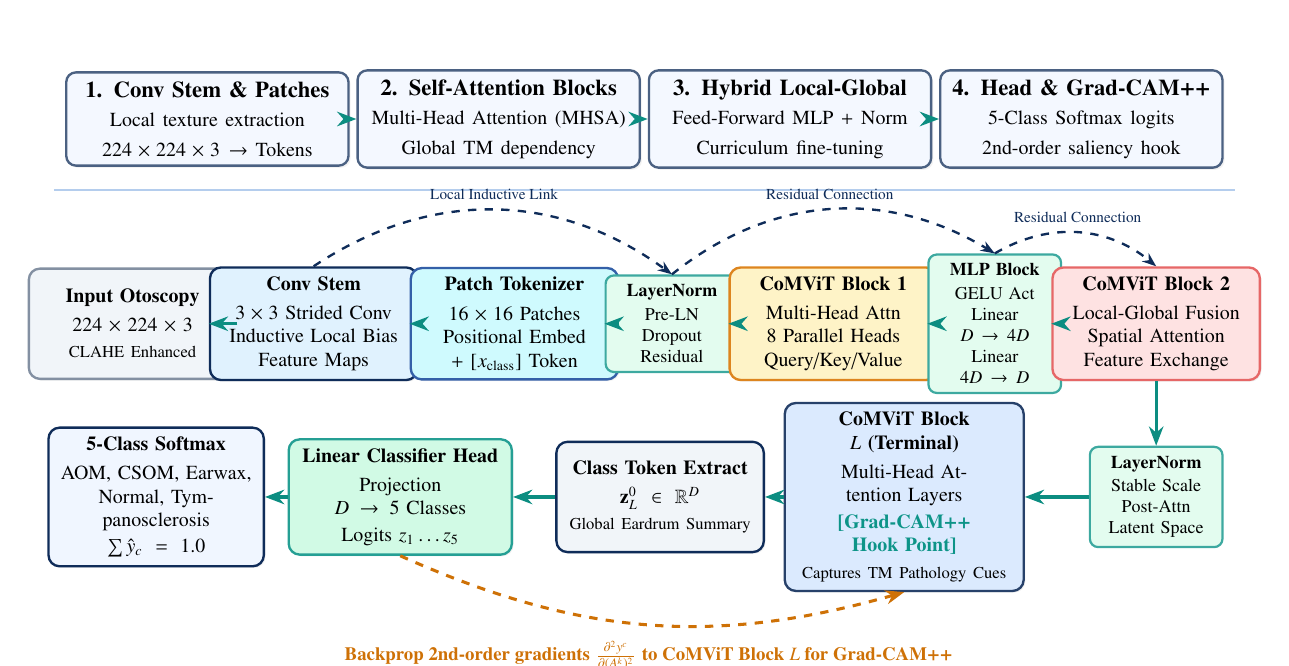
\begin{tikzpicture}[
  x=1cm, y=1cm,
  font=\sffamily,
  dagstep/.style={rectangle, rounded corners=3.5pt, minimum height=1.10cm,
    text width=3.35cm, align=center, draw=lavenderDark!75, fill=lavenderLight!75,
    line width=0.85pt, font=\fontsize{8.2}{9.8}\selectfont\bfseries,
    drop shadow={shadow xshift=0.8pt, shadow yshift=-0.8pt, opacity=0.10}},
  dagarrow/.style={-{Stealth[scale=0.85]}, line width=1.15pt, draw=prismTeal!95!black},
  blkbox/.style={rectangle, rounded corners=4pt, line width=0.85pt,
    minimum height=1.40cm, text width=2.40cm, align=center,
    font=\fontsize{7.2}{8.5}\selectfont, drop shadow={shadow xshift=0.6pt, shadow yshift=-0.6pt, opacity=0.12}},
  transbox/.style={rectangle, rounded corners=3pt, line width=0.80pt,
    draw=prismTeal!80, fill=cStage1!60, minimum height=1.15cm, text width=1.45cm, align=center,
    font=\fontsize{6.5}{7.6}\selectfont},
  skipconn/.style={-{Stealth[scale=0.75]}, line width=0.85pt, draw=prismNavy, dashed}
]

  % Row 1: 4-Stage Architectural Progression
  \node[dagstep] (s1) at (-5.55, 0) {1. Conv Stem \& Patches\\[2pt]\normalfont\fontsize{7.2}{8.5}\selectfont Local texture extraction\\[1pt]$224\times 224\times 3 \to$ Tokens};
  \node[dagstep] (s2) at (-1.85, 0) {2. Self-Attention Blocks\\[2pt]\normalfont\fontsize{7.2}{8.5}\selectfont Multi-Head Attention (MHSA)\\[1pt]Global TM dependency};
  \node[dagstep] (s3) at (1.85, 0) {3. Hybrid Local-Global\\[2pt]\normalfont\fontsize{7.2}{8.5}\selectfont Feed-Forward MLP + Norm\\[1pt]Curriculum fine-tuning};
  \node[dagstep] (s4) at (5.55, 0) {4. Head \& Grad-CAM++\\[2pt]\normalfont\fontsize{7.2}{8.5}\selectfont 5-Class Softmax logits\\[1pt]2nd-order saliency hook};

  \draw[dagarrow] (s1) -- (s2);
  \draw[dagarrow] (s2) -- (s3);
  \draw[dagarrow] (s3) -- (s4);

  % Separator
  \draw[draw=lavenderBorder, line width=0.6pt] (-7.5, -0.90) -- (7.5, -0.90);

  % Row 2 & 3: Detailed Layer Decomposition Flow
  \node[blkbox, fill=cInput, draw=prismSlate!80] (input_node) at (-6.50, -2.60) {
    \textbf{Input Otoscopy}\\[2pt]
    $224\times 224\times 3$\\[1pt]
    {\fontsize{6.0}{7.0}\selectfont CLAHE Enhanced}
  };

  \node[blkbox, fill=cStem, draw=lavenderDark] (stem_node) at (-4.20, -2.60) {
    \textbf{Conv Stem}\\[2pt]
    $3\times 3$ Strided Conv\\
    Inductive Local Bias\\
    Feature Maps
  };

  \node[blkbox, fill=cStage4, draw=prismBlue!90] (token_node) at (-1.65, -2.60) {
    \textbf{Patch Tokenizer}\\[2pt]
    $16\times 16$ Patches\\
    Positional Embed\\
    + $[x_{\text{class}}]$ Token
  };

  \node[transbox] (tr1) at (0.35, -2.60) {
    \textbf{LayerNorm}\\[1pt]
    Pre-LN\\
    Dropout\\
    Residual
  };

  \node[blkbox, fill=cStage2, draw=prismGold!90] (vit1) at (2.40, -2.60) {
    \textbf{CoMViT Block 1}\\[2pt]
    Multi-Head Attn\\
    8 Parallel Heads\\
    Query/Key/Value
  };

  \node[transbox] (tr2) at (4.45, -2.60) {
    \textbf{MLP Block}\\[1pt]
    GELU Act\\
    Linear $D\to 4D$\\
    Linear $4D\to D$
  };

  \node[blkbox, fill=cStage3, draw=statusFail!70] (vit2) at (6.50, -2.60) {
    \textbf{CoMViT Block 2}\\[2pt]
    Local-Global Fusion\\
    Spatial Attention\\
    Feature Exchange
  };

  % Second Row of Layers
  \node[transbox] (tr3) at (6.50, -4.80) {
    \textbf{LayerNorm}\\[1pt]
    Stable Scale\\
    Post-Attn\\
    Latent Space
  };

  \node[blkbox, fill=cHead, draw=lavenderDark!90, text width=2.80cm] (vitL) at (3.30, -4.80) {
    \textbf{CoMViT Block $L$ (Terminal)}\\[2pt]
    Multi-Head Attention Layers\\[1pt]
    {\color{prismTeal}\textbf{[Grad-CAM++ Hook Point]}}\\[1pt]
    {\fontsize{6.0}{7.0}\selectfont Captures TM Pathology Cues}
  };

  \node[blkbox, fill=cInput, draw=prismNavy] (cls_token) at (0.20, -4.80) {
    \textbf{Class Token Extract}\\[2pt]
    $\mathbf{z}_L^0 \in \mathbb{R}^D$\\[1pt]
    {\fontsize{6.0}{7.0}\selectfont Global Eardrum Summary}
  };

  \node[blkbox, fill=cStage1, draw=prismTeal!90, text width=2.60cm] (head) at (-3.10, -4.80) {
    \textbf{Linear Classifier Head}\\[2pt]
    Projection $D \to 5$ Classes\\[1pt]
    Logits $z_1 \dots z_5$
  };

  \node[blkbox, fill=lavenderLight, draw=lavenderDark, text width=2.50cm] (softmax) at (-6.20, -4.80) {
    \textbf{5-Class Softmax}\\[2pt]
    AOM, CSOM, Earwax,\\
    Normal, Tympanosclerosis\\[1pt]
    $\sum \hat{y}_c = 1.0$
  };

  % Forward Flow Connections
  \draw[dagarrow] (input_node) -- (stem_node);
  \draw[dagarrow] (stem_node) -- (token_node);
  \draw[dagarrow] (token_node) -- (tr1);
  \draw[dagarrow] (tr1) -- (vit1);
  \draw[dagarrow] (vit1) -- (tr2);
  \draw[dagarrow] (tr2) -- (vit2);
  \draw[dagarrow] (vit2) -- (tr3);
  \draw[dagarrow] (tr3) -- (vitL);
  \draw[dagarrow] (vitL) -- (cls_token);
  \draw[dagarrow] (cls_token) -- (head);
  \draw[dagarrow] (head) -- (softmax);

  % Skip Connections
  \draw[skipconn] (stem_node.north) to[bend left=35] node[above, font=\fontsize{5.5}{6.5}\selectfont\color{prismNavy}]{Local Inductive Link} (tr1.north);
  \draw[skipconn] (tr1.north) to[bend left=35] node[above, font=\fontsize{5.5}{6.5}\selectfont\color{prismNavy}]{Residual Connection} (tr2.north);
  \draw[skipconn] (tr2.north) to[bend left=35] node[above, font=\fontsize{5.5}{6.5}\selectfont\color{prismNavy}]{Residual Connection} (vit2.north);

  % Backward Hook Arrow
  \draw[-{Stealth[scale=0.85]}, line width=1.1pt, draw=prismGold!95!black, dashed] 
    (head.south) to[bend right=20] 
    node[below=2pt, font=\fontsize{6.8}{8.0}\selectfont\bfseries\color{prismGold!95!black}]{Backprop 2nd-order gradients $\frac{\partial^2 y^c}{\partial (A^k)^2}$ to CoMViT Block $L$ for Grad-CAM++} 
    (vitL.south);

\end{tikzpicture}
\end{document}
}
    \caption{CoMViT architecture decomposition graph illustrating convolutional patch stem, Multi-Head Self-Attention blocks, latent token representations, 5-class linear classifier, and Grad-CAM++ backward hook point.}
    \label{fig:dag_scheduling_walkthrough}
\end{figure}

\section{Detailed Component Analysis}

\subsection{Data Storage, Model Artifacts, and Schema Connectors}
Figure~\ref{fig:db_schema} depicts the relational schema connecting dataset partitions, curriculum training configurations, CoMViT model checkpoints, evaluation telemetry, and API contract payloads.

\begin{figure}[H]
    \centering
    \adjustbox{max width=0.98\linewidth, max height=0.72\textheight, keepaspectratio, center}{\documentclass[tikz,border=10pt]{standalone}
\usepackage{tikz}
\usepackage{fontawesome5}
\usepackage{amsmath,amssymb}
\usetikzlibrary{arrows.meta,positioning,fit,backgrounds,calc,shadows,shapes.geometric}

% Color definitions
\definecolor{lavenderDark}{RGB}{15, 44, 89}
\definecolor{lavenderDeep}{RGB}{10, 28, 58}
\definecolor{lavenderMedium}{RGB}{29, 78, 158}
\definecolor{lavenderLight}{RGB}{240, 246, 255}
\definecolor{lavenderBorder}{RGB}{180, 205, 237}
\definecolor{prismTeal}{RGB}{13, 148, 136}
\definecolor{prismMint}{RGB}{236, 253, 245}
\definecolor{prismGold}{RGB}{217, 119, 6}
\definecolor{prismDark}{RGB}{15, 23, 42}
\definecolor{cInput}{RGB}{241, 245, 249}
\definecolor{cPlanner}{RGB}{219, 234, 254}
\definecolor{cReact}{RGB}{209, 250, 229}
\definecolor{cTool}{RGB}{254, 243, 199}
\definecolor{cSafety}{RGB}{254, 226, 226}
\definecolor{cDeliverable}{RGB}{204, 251, 241}

\begin{document}
% Relational Entity & Storage Schema Connectors for Ear Disease Detection
\begin{tikzpicture}[
  x=1cm, y=1cm,
  font=\sffamily,
  tblcard/.style={
    rectangle, rounded corners=4pt, draw=lavenderDark!75, line width=0.85pt, fill=white,
    inner sep=5pt, text width=4.40cm, align=left,
    drop shadow={shadow xshift=1pt, shadow yshift=-1pt, opacity=0.12}
  },
  fkarrow/.style={
    -{Stealth[scale=0.85]}, line width=1.0pt, draw=lavenderDark!90
  },
  fklabel/.style={
    font=\fontsize{6.2}{7.2}\selectfont\bfseries, fill=white, inner sep=1.5pt, text=lavenderDark
  }
]

  % ================= COLUMN 1: DATASET & CONFIGURATION (x = -5.2) =================
  
  % Table 1: merged_otoscopic_dataset_store
  \node[tblcard] (dataset) at (-5.2, 2.5) {%
    \centerline{\color{lavenderDark}\faFolderOpen\ \textbf{\fontsize{8.0}{9.5}\selectfont merged\_otoscopic\_dataset}}\\[3pt]
    \rule{\linewidth}{0.4pt}\\[3pt]
    {\fontsize{6.8}{8.0}\selectfont
    \textbf{\color{lavenderDark}[PK]} \texttt{image\_id}: \textit{string} (Indexed)\\
    \textbf{\color{prismTeal}[FLD]} \texttt{class\_label}: \textit{AOM/CSOM/WAX/NORM/TS}\\
    \textbf{\color{prismDark!80}[FLD]} \texttt{split}: \textit{train / val / test (Curriculum)}\\
    \textbf{\color{prismDark!80}[FLD]} \texttt{clahe\_enhanced}: \textit{boolean (true)}\\
    \textbf{\color{prismDark!80}[FLD]} \texttt{tensor\_dims}: \textit{$(3, 224, 224)$ normalized}}
  };

  % Table 2: training_curriculum_store
  \node[tblcard, below=0.70cm of dataset] (config) {%
    \centerline{\color{lavenderDark}\faCogs\ \textbf{\fontsize{8.0}{9.5}\selectfont training\_curriculum\_store}}\\[3pt]
    \rule{\linewidth}{0.4pt}\\[3pt]
    {\fontsize{6.8}{8.0}\selectfont
    \textbf{\color{lavenderDark}[PK]} \texttt{config\_id}: \textit{string} (UUID)\\
    \textbf{\color{prismDark!80}[FLD]} \texttt{image\_size}: \textit{224} $\cdot$ \texttt{batch\_size}: \textit{32}\\
    \textbf{\color{prismDark!80}[FLD]} \texttt{mixup\_alpha}: \textit{0.2 (Beta distribution)}\\
    \textbf{\color{prismDark!80}[FLD]} \texttt{pacing\_rate}: \textit{adaptive curriculum}\\
    \textbf{\color{prismDark!80}[FLD]} \texttt{optimizer}: \textit{AdamW} ($\eta=10^{-4}$)\\
    \textbf{\color{prismDark!80}[FLD]} \texttt{augmentations}: \textit{CLAHE, rot, flip, affine}}
  };

  % ================= COLUMN 2: MODEL CHECKPOINTS & EVALUATION (x = 0) =================
  
  % Table 3: comvit_model_store
  \node[tblcard] (checkpoint) at (0, 2.5) {%
    \centerline{\color{lavenderDark}\faDatabase\ \textbf{\fontsize{8.0}{9.5}\selectfont comvit\_model\_store}}\\[3pt]
    \rule{\linewidth}{0.4pt}\\[3pt]
    {\fontsize{6.8}{8.0}\selectfont
    \textbf{\color{lavenderDark}[PK]} \texttt{checkpoint\_id}: \textit{timestamp}\\
    \textbf{\color{prismTeal}[FK]} \texttt{config\_id}: \textit{curriculum ref}\\
    \textbf{\color{prismDark!80}[FLD]} \texttt{architecture}: \textit{CoMViT (Hybrid ViT)}\\
    \textbf{\color{prismDark!80}[FLD]} \texttt{target\_classes}: \textit{5 disease categories}\\
    \textbf{\color{prismDark!80}[FLD]} \texttt{weights\_path}: \textit{comvit\_ear\_best.pth}\\
    \textbf{\color{prismDark!80}[FLD]} \texttt{classes\_file}: \textit{disease\_labels.json}}
  };

  % Table 4: evaluation_telemetry_store
  \node[tblcard, below=0.70cm of checkpoint] (eval) {%
    \centerline{\color{lavenderDark}\faChartLine\ \textbf{\fontsize{8.0}{9.5}\selectfont evaluation\_telemetry\_store}}\\[3pt]
    \rule{\linewidth}{0.4pt}\\[3pt]
    {\fontsize{6.8}{8.0}\selectfont
    \textbf{\color{lavenderDark}[PK]} \texttt{eval\_id}: \textit{UUID}\\
    \textbf{\color{prismTeal}[FK]} \texttt{checkpoint\_id}: \textit{model reference}\\
    \textbf{\color{prismDark!80}[FLD]} \texttt{multi\_class\_acc}: \textit{test benchmark}\\
    \textbf{\color{prismDark!80}[FLD]} \texttt{macro\_f1}: \textit{harmonic mean}\\
    \textbf{\color{prismDark!80}[FLD]} \texttt{roc\_auc\_ovr}: \textit{one-vs-rest AUC}\\
    \textbf{\color{prismDark!80}[FLD]} \texttt{class\_metrics}: \textit{AOM, CSOM, Wax, Norm, TS}}
  };

  % ================= COLUMN 3: API CONTRACTS & CLIENT STATE (x = 5.2) =================
  
  % Table 5: api_prediction_schema
  \node[tblcard] (prediction) at (5.2, 2.5) {%
    \centerline{\color{lavenderDark}\faServer\ \textbf{\fontsize{8.0}{9.5}\selectfont api\_prediction\_schema}}\\[3pt]
    \rule{\linewidth}{0.4pt}\\[3pt]
    {\fontsize{6.8}{8.0}\selectfont
    \textbf{\color{lavenderDark}[PK]} \texttt{prediction\_id}: \textit{UUID}\\
    \textbf{\color{prismTeal}[FK]} \texttt{checkpoint\_id}: \textit{active CoMViT}\\
    \textbf{\color{prismDark!80}[FLD]} \texttt{success}: \textit{boolean (true)}\\
    \textbf{\color{prismDark!80}[FLD]} \texttt{predicted\_class}: \textit{5 classes}\\
    \textbf{\color{prismDark!80}[FLD]} \texttt{confidence}: \textit{float (0.0 .. 1.0)}\\
    \textbf{\color{prismDark!80}[FLD]} \texttt{probabilities}: \textit{5-class JSON map}\\
    \textbf{\color{prismDark!80}[FLD]} \texttt{processing\_time\_ms}: \textit{float ($\le 50$\,ms)}\\
    \textbf{\color{prismDark!80}[FLD]} \texttt{safety\_notice}: \textit{ENT decision support}}
  };

  % Table 6: client_ui_state_schema
  \node[tblcard, below=0.70cm of prediction] (client) {%
    \centerline{\color{lavenderDark}\faDesktop\ \textbf{\fontsize{8.0}{9.5}\selectfont client\_ui\_state\_schema}}\\[3pt]
    \rule{\linewidth}{0.4pt}\\[3pt]
    {\fontsize{6.8}{8.0}\selectfont
    \textbf{\color{lavenderDark}[PK]} \texttt{session\_id}: \textit{UUID}\\
    \textbf{\color{prismTeal}[FK]} \texttt{prediction\_id}: \textit{payload reference}\\
    \textbf{\color{prismDark!80}[FLD]} \texttt{otoscopy\_preview}: \textit{blob/base64}\\
    \textbf{\color{prismDark!80}[FLD]} \texttt{gradcam\_pp\_map}: \textit{PNG TM overlay}\\
    \textbf{\color{prismDark!80}[FLD]} \texttt{visual\_probabilities}: \textit{5-class bar chart}\\
    \textbf{\color{prismDark!80}[FLD]} \texttt{client\_platform}: \textit{Web / Mobile Otoscope}}
  };

  % ================= RELATIONSHIPS / FOREIGN KEY CONNECTORS =================

  % 1. Config -> Checkpoint
  \draw[fkarrow] (config.east) to[bend right=20] 
    node[above=1pt, fklabel]{config\_id} (checkpoint.west);

  % 2. Dataset -> Checkpoint (Data used to train)
  \draw[fkarrow] (dataset.east) -- 
    node[above=1pt, fklabel]{curriculum\_split} (checkpoint.west);

  % 3. Checkpoint -> Evaluation
  \draw[fkarrow] (checkpoint.south) -- 
    node[right=2pt, fklabel]{checkpoint\_id} (eval.north);

  % 4. Checkpoint -> API Prediction
  \draw[fkarrow] (checkpoint.east) -- 
    node[above=1pt, fklabel]{weights} (prediction.west);

  % 5. API Prediction -> Client UI State
  \draw[fkarrow] (prediction.south) -- 
    node[right=2pt, fklabel]{prediction\_id} (client.north);

  % 6. Eval metrics reference in Client UI
  \draw[fkarrow, dashed] (eval.east) -- 
    node[above=1pt, fklabel]{benchmarks} (client.west);

\end{tikzpicture}
\end{document}
}
    \caption{Relational entity and data storage schema connectors showing merged otoscopic dataset, training curriculum configurations, CoMViT model checkpoints, evaluation telemetry, and API contract specifications.}
    \label{fig:db_schema}
\end{figure}

\subsection{Level-1 Data Flow Architecture}
Figure~\ref{fig:data_flow_diagram} presents the Level-1 Data Flow Diagram (DFD), showing external entities, primary processing transformations, datastores, and explainability feedback loops.

\begin{figure}[H]
    \centering
    \adjustbox{max width=0.98\linewidth, max height=0.72\textheight, keepaspectratio, center}{\documentclass[tikz,border=10pt]{standalone}
\usepackage{tikz}
\usepackage{amsmath,amssymb}
\usepackage{fontawesome5}
\usetikzlibrary{arrows.meta,positioning,fit,backgrounds,calc,shadows,shapes.geometric}

% Color definitions
\definecolor{lavenderDark}{RGB}{15, 44, 89}
\definecolor{lavenderDeep}{RGB}{10, 28, 58}
\definecolor{lavenderMedium}{RGB}{29, 78, 158}
\definecolor{lavenderLight}{RGB}{240, 246, 255}
\definecolor{lavenderBorder}{RGB}{180, 205, 237}
\definecolor{prismNavy}{RGB}{15, 44, 89}
\definecolor{prismBlue}{RGB}{29, 78, 158}
\definecolor{prismTeal}{RGB}{13, 148, 136}
\definecolor{prismGold}{RGB}{217, 119, 6}
\definecolor{prismDark}{RGB}{15, 23, 42}
\definecolor{cInput}{RGB}{241, 245, 249}
\definecolor{cStem}{RGB}{224, 242, 254}
\definecolor{cStage1}{RGB}{209, 250, 229}
\definecolor{cStage2}{RGB}{254, 243, 199}
\definecolor{cStage4}{RGB}{207, 250, 254}
\definecolor{cHead}{RGB}{219, 234, 254}

\begin{document}
% Level-1 Data Flow Diagram (DFD) for Ear Disease Detection
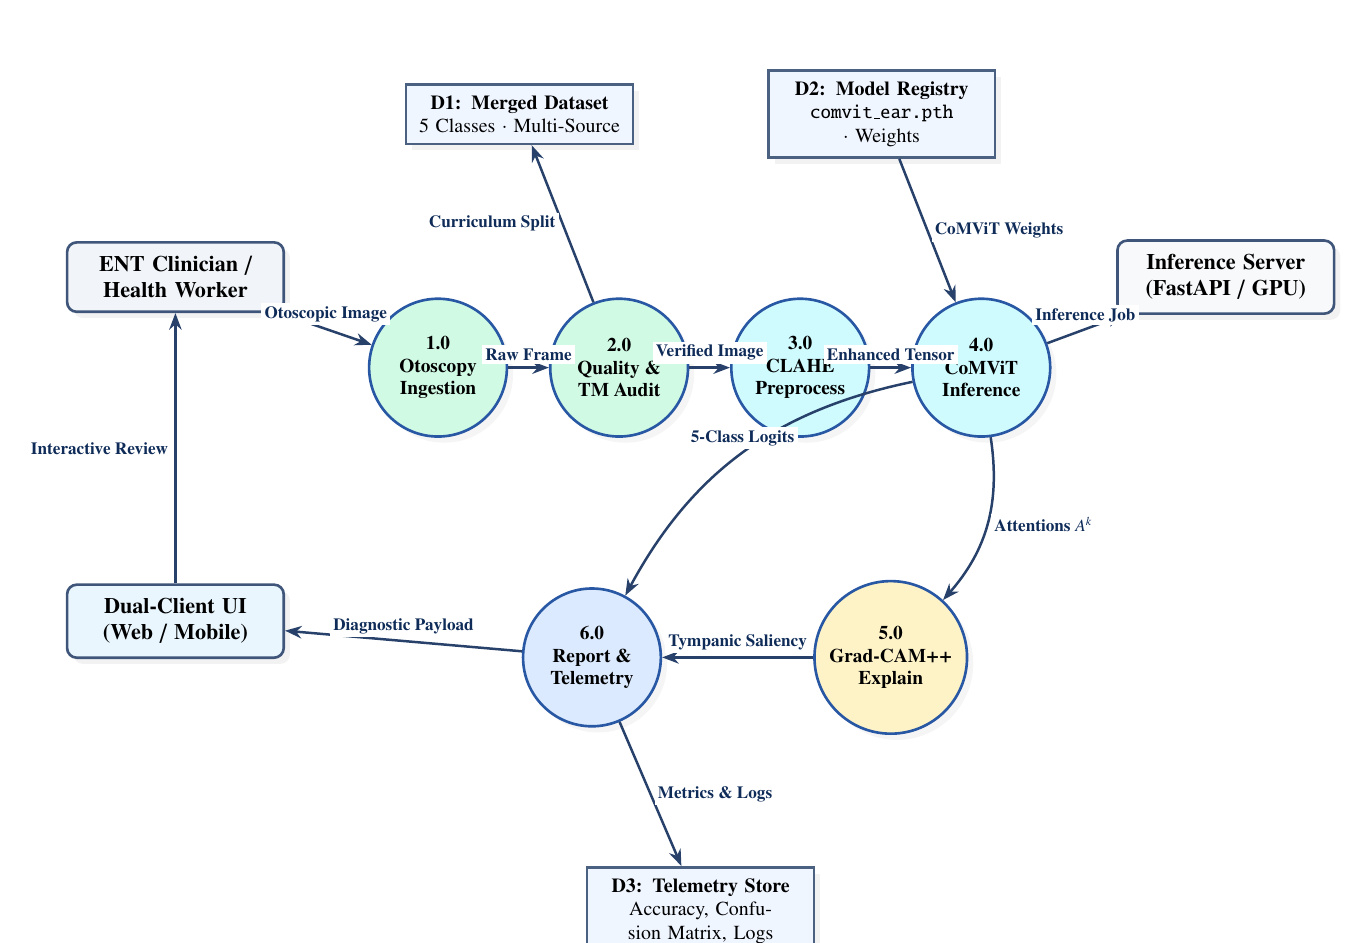
\begin{tikzpicture}[
  x=1.15cm, y=1.15cm,
  font=\sffamily,
  entity/.style={
    rectangle, draw=lavenderDark!80, line width=0.95pt, rounded corners=3.5pt,
    align=center, inner sep=5pt, font=\fontsize{8.0}{9.5}\selectfont\bfseries,
    text width=2.40cm, fill=cInput, drop shadow={opacity=0.10}
  },
  store/.style={
    rectangle, draw=lavenderDark!75, line width=0.95pt,
    align=center, inner sep=4.0pt, font=\fontsize{7.2}{8.5}\selectfont,
    text width=2.60cm, fill=lavenderLight, drop shadow={opacity=0.10}
  },
  proc/.style={
    circle, draw=lavenderMedium!95, line width=0.95pt,
    align=center, inner sep=2pt, minimum size=1.75cm,
    font=\fontsize{7.0}{8.2}\selectfont\bfseries, fill=cStage1, drop shadow={opacity=0.08}
  },
  procblue/.style={proc, fill=cStage4},
  procgold/.style={proc, fill=cStage2},
  prochead/.style={proc, fill=cHead},
  dfdarr/.style={
    -{Stealth[scale=0.85]}, line width=0.90pt, draw=lavenderDark!90
  },
  flowlbl/.style={
    font=\fontsize{6.2}{7.2}\selectfont\bfseries, fill=white, inner sep=1.2pt, text=lavenderDark
  }
]

  % External Entities
  \node[entity] (user) at (-5.8, 3.2) {ENT Clinician /\\Health Worker};
  \node[entity, fill=cStem!70] (client_ui) at (-5.8, -0.6) {Dual-Client UI\\(Web / Mobile)};
  \node[entity, fill=cInput!60] (host_server) at (5.8, 3.2) {Inference Server\\(FastAPI / GPU)};

  % Data Stores
  \node[store] (d1) at (-2.0, 5.0) {\textbf{D1: Merged Dataset}\\ 5 Classes $\cdot$ Multi-Source};
  \node[store] (d2) at (2.0, 5.0) {\textbf{D2: Model Registry}\\ \texttt{comvit\_ear.pth} $\cdot$ Weights};
  \node[store] (d3) at (0.0, -3.8) {\textbf{D3: Telemetry Store}\\ Accuracy, Confusion Matrix, Logs};

  % Core DFD Processes
  \node[proc] (p1) at (-2.9, 2.2) {1.0\\Otoscopy\\Ingestion};
  \node[proc] (p2) at (-0.9, 2.2) {2.0\\Quality \&\\TM Audit};
  \node[procblue] (p3) at (1.1, 2.2) {3.0\\CLAHE\\Preprocess};
  \node[procblue] (p4) at (3.1, 2.2) {4.0\\CoMViT\\Inference};

  \node[procgold] (p5) at (2.1, -1.0) {5.0\\Grad-CAM++\\Explain};
  \node[prochead] (p6) at (-1.2, -1.0) {6.0\\Report \&\\Telemetry};

  % Flow Connections: Ingestion Pipeline
  \draw[dfdarr] (user) -- node[above=1pt, flowlbl]{Otoscopic Image} (p1);
  \draw[dfdarr] (p1) -- node[above=1pt, flowlbl]{Raw Frame} (p2);
  \draw[dfdarr] (p2) -- node[left=1pt, flowlbl]{Curriculum Split} (d1);
  \draw[dfdarr] (p2) -- node[above=1pt, flowlbl]{Verified Image} (p3);
  \draw[dfdarr] (p3) -- node[above=1pt, flowlbl]{Enhanced Tensor} (p4);

  % Model Weights Fetch
  \draw[dfdarr] (d2) -- node[right=1pt, flowlbl]{CoMViT Weights} (p4);
  \draw[dfdarr] (p4) -- node[above=1pt, flowlbl]{Inference Job} (host_server);

  % Inference to Grad-CAM++ and Report
  \draw[dfdarr] (p4) to[bend left=25] node[right=1pt, flowlbl]{Attentions $A^k$} (p5);
  \draw[dfdarr] (p4) to[bend right=25] node[above=1pt, flowlbl]{5-Class Logits} (p6);
  \draw[dfdarr] (p5) -- node[above=1pt, flowlbl]{Tympanic Saliency} (p6);

  % Report to Client UI and Telemetry
  \draw[dfdarr] (p6) -- node[above=1pt, flowlbl]{Diagnostic Payload} (client_ui);
  \draw[dfdarr] (p6) -- node[right=1pt, flowlbl]{Metrics \& Logs} (d3);
  \draw[dfdarr] (client_ui) -- node[left=1pt, flowlbl]{Interactive Review} (user);

\end{tikzpicture}
\end{document}
}
    \caption{Level-1 Data Flow Diagram (DFD) depicting external entities, validation and inference processing transformations, datastores, and explainability feedback loops.}
    \label{fig:data_flow_diagram}
\end{figure}


%==============================================================================
% CHAPTER 6: DESIGN AND METHODOLOGY
%==============================================================================
\chapter{Design and Methodology}

This chapter details the mathematical foundations of CoMViT and Grad-CAM++, CLAHE contrast enhancement, controlled MixUp, adaptive curriculum learning, benchmark dataset curation, FastAPI serving, and empirical evaluation metrics.

\section{Mathematical Foundations of CoMViT and Grad-CAM++}

\subsection{CoMViT Hybrid Inductive Architecture}
Pure Vision Transformers treat images as non-overlapping patches, lacking the translation equivariance and local locality priors inherent to convolutions. CoMViT remedies this by incorporating a shallow convolutional stem that processes the input image tensor $\mathbf{x} \in \mathbb{R}^{3 \times 224 \times 224}$:
\begin{equation}
    \mathbf{F}_0 = \mathrm{ConvStem}(\mathbf{x}) \in \mathbb{R}^{C_{\text{stem}} \times \frac{H}{P} \times \frac{W}{P}}
\end{equation}
The feature maps are flattened into spatial tokens and linearly projected to embedding dimension $D$. A learnable classification token $\mathbf{x}_{\text{class}} \in \mathbb{R}^D$ and 1D learnable positional encodings $\mathbf{E}_{\text{pos}} \in \mathbb{R}^{(N+1) \times D}$ are prepended:
\begin{equation}
    \mathbf{z}_0 = [\mathbf{x}_{\text{class}}; \, \mathbf{F}_0^1 \mathbf{W}_E; \, \dots; \, \mathbf{F}_0^N \mathbf{W}_E] + \mathbf{E}_{\text{pos}}
\end{equation}
The sequence passes through $L$ transformer encoder blocks:
\begin{align}
    \mathbf{z}'_l &= \mathrm{MHSA}\big(\mathrm{LayerNorm}(\mathbf{z}_{l-1})\big) + \mathbf{z}_{l-1} \\
    \mathbf{z}_l &= \mathrm{MLP}\big(\mathrm{LayerNorm}(\mathbf{z}'_l)\big) + \mathbf{z}'_l
\end{align}
where the Multi-Head Self-Attention operates across $h=8$ parallel heads, computing dot-product affinities between all patch pairs. This enables CoMViT to simultaneously preserve localized micro-textures (vascularity, erythema, plaque edges) and global eardrum morphology (annulus integrity, malleus position).

\subsection{Grad-CAM++ Higher-Order Gradient Formulation}
To address the coarse resolution and localization failures of standard Grad-CAM when multiple lesions or complex pathology borders are present, Grad-CAM++ incorporates second- and third-order partial derivatives. For target class score $Y^c = \exp(z_c)$ and feature activation map $A^k$ at spatial coordinate $(i, j)$:
\begin{equation}
    \alpha_{ijk}^c = \frac{\frac{\partial^2 Y^c}{(\partial A_{ij}^k)^2}}{2\frac{\partial^2 Y^c}{(\partial A_{ij}^k)^2} + \sum_{a=1}^U \sum_{b=1}^V A_{ab}^k \left( \frac{\partial^3 Y^c}{(\partial A_{ij}^k)^3} \right)}
\end{equation}
The class-discriminative weight $w_k^c$ is computed by summing over positive gradients:
\begin{equation}
    w_k^c = \sum_{i=1}^U \sum_{j=1}^V \alpha_{ijk}^c \cdot \mathrm{ReLU}\left( \frac{\partial Y^c}{\partial A_{ij}^k} \right)
\end{equation}
The final 2D saliency map $L_{\text{Grad-CAM++}}^c \in \mathbb{R}^{U \times V}$ is generated as:
\begin{equation}
    L_{\text{Grad-CAM++}}^c = \mathrm{ReLU}\left( \sum_{k=1}^K w_k^c A^k \right)
\end{equation}
Upsampling $L_{\text{Grad-CAM++}}^c$ to $224 \times 224$ via bilinear interpolation and blending with a Jet colormap overlay produces a clinically precise heatmap that pinpoints exact pathological regions on the tympanic membrane.

\section{Data Preparation and Benchmark Dataset Curation}
The benchmark dataset was constructed by merging publicly available and verified clinical otoscopic and eardrum imaging datasets, harmonizing them into five distinct pathological categories:
\begin{itemize}
    \item \textbf{Acute Otitis Media (AOM):} Characterized by intense hyperemic erythema, significant eardrum bulging, loss of normal light reflex, and opaque purulent middle ear effusion.
    \item \textbf{Chronic Suppurative Otitis Media (CSOM):} Characterized by visible central or marginal tympanic membrane perforations in the pars tensa, purulent or mucoid otorrhea, and mucosal thickening.
    \item \textbf{Earwax (Cerumen Impaction):} Partial or total occlusion of the external auditory canal by dark brown or golden cerumen deposits obstructing visualization of the underlying tympanic membrane.
    \item \textbf{Normal:} Translucent, pearl-gray, concave tympanic membrane with distinct visualization of the malleus handle, umbo, and prominent anterior-inferior cone of light.
    \item \textbf{Tympanosclerosis:} Distinct chalky-white, dense calcareous plaques embedded within the tympanic membrane laminae without active acute inflammation or perforation.
\end{itemize}

Every image was validated through PIL byte-checking to eliminate corrupt files. Contrast Limited Adaptive Histogram Equalization (CLAHE) was applied to rectify non-uniform illumination and accentuate morphological contours, followed by resizing to $224 \times 224$ pixels and channel standardization. The dataset was partitioned into 70\% training, 15\% validation, and 15\% testing splits using stratified sampling.

\section{Multi-Stage Machine Learning Pipeline Design}

\subsection{Training Protocol and Hyperparameters}
The CoMViT model was trained using AdamW optimization with decoupled weight decay. Controlled MixUp augmentation ($\alpha = 0.20$) and adaptive curriculum pacing were applied during training. Hyperparameters are detailed in Table~\ref{tab:ml_hyperparameters}.

\begin{table}[H]
\centering
\caption{CoMViT Training Configuration and Hyperparameters.}
\label{tab:ml_hyperparameters}
\small
\begin{tabularx}{\textwidth}{l p{4.2cm} X}
\toprule
\textbf{Component} & \textbf{Parameter Name} & \textbf{Configured Value / Rationale} \\
\midrule
Image Resolution & \texttt{image\_size} & $224 \times 224 \times 3$ (Standardized input resolution) \\
Batch Size & \texttt{batch\_size} & 32 (Stable gradient estimation and memory efficiency) \\
Optimizer & Type & AdamW (Decoupled weight decay, $\beta_1=0.9, \beta_2=0.999$) \\
Learning Rate & \texttt{learning\_rate} & $10^{-4}$ with cosine annealing schedule \\
Weight Decay & \texttt{weight\_decay} & $10^{-4}$ (L2 regularization preventing parameter divergence) \\
MixUp Coefficient & \texttt{mixup\_alpha} & $\alpha = 0.20$ (Beta distribution for convex sample mixing) \\
Epochs & \texttt{epochs} & 35 epochs maximum \\
Early Stopping & \texttt{patience} & 7 epochs on validation loss \\
Augmentations & Transformations & CLAHE, random flips ($p=0.5$), rotation ($\pm 15^\circ$), affine scaling \\
\bottomrule
\end{tabularx}
\end{table}

\subsection{Model Responsibilities and Staged Inference Flow}
Figure~\ref{fig:ml_inference_flow} maps the six specialized operational stages executed during inference.

\begin{figure}[H]
    \centering
    \adjustbox{max width=0.98\linewidth, max height=0.72\textheight, keepaspectratio, center}{\documentclass[tikz,border=10pt]{standalone}
\usepackage{tikz}
\usepackage{fontawesome5}
\usepackage{amsmath,amssymb}
\usetikzlibrary{arrows.meta,positioning,fit,backgrounds,calc,shadows,shapes.geometric}

% Color definitions
\definecolor{lavenderDark}{RGB}{15, 44, 89}
\definecolor{lavenderDeep}{RGB}{10, 28, 58}
\definecolor{lavenderMedium}{RGB}{29, 78, 158}
\definecolor{lavenderLight}{RGB}{240, 246, 255}
\definecolor{lavenderBorder}{RGB}{180, 205, 237}
\definecolor{prismNavy}{RGB}{15, 44, 89}
\definecolor{prismBlue}{RGB}{29, 78, 158}
\definecolor{prismTeal}{RGB}{13, 148, 136}
\definecolor{prismGold}{RGB}{217, 119, 6}
\definecolor{prismDark}{RGB}{15, 23, 42}
\definecolor{cInput}{RGB}{241, 245, 249}
\definecolor{cStem}{RGB}{224, 242, 254}
\definecolor{cStage1}{RGB}{209, 250, 229}
\definecolor{cStage2}{RGB}{254, 243, 199}
\definecolor{cStage4}{RGB}{207, 250, 254}
\definecolor{cHead}{RGB}{219, 234, 254}

\begin{document}
% Model Responsibilities & Staged Inference Flow for Ear Disease Detection
\begin{tikzpicture}[
    x=1cm, y=1cm, font=\sffamily,
    modelrow/.style={rectangle, rounded corners=3.5pt, draw=lavenderDark!45,
      line width=0.65pt, inner sep=4.5pt},
    arrow/.style={-{Stealth[scale=0.8]}, line width=0.9pt, draw=lavenderDark!85}
]

  % Stage 1: Input Validation (y = 0.0)
  \node[modelrow, fill=cInput!70, text width=2.40cm, align=center, minimum height=1.15cm] (m1l) at (-5.85, 0.0)
    {{\fontsize{8.5}{10.2}\selectfont\color{lavenderDark}\faCheckCircle\ \textbf{1. Validation}}\\[2pt]
     {\fontsize{7.5}{9.0}\selectfont\texttt{otoscopy\_guard}}};
  \node[modelrow, fill=lavenderLight!85, text width=7.40cm, align=left, minimum height=1.15cm] (m1p) at (-0.55, 0.0)
    {\fontsize{7.6}{9.0}\selectfont \textbf{Payload Audit} $\rightarrow$ Verify MIME in \{JPEG, PNG, BMP\}\\[2pt]Validate payload size $\le 10$\,MB $\rightarrow$ Eardrum presence / cerumen audit};
  \node[modelrow, fill=lavenderLight!85, text width=4.10cm, align=left, minimum height=1.15cm] (m1r) at (5.60, 0.0)
    {\fontsize{7.6}{9.0}\selectfont \textbf{Sanitized Byte Stream}\\[2pt]{\fontsize{6.8}{8.0}\selectfont Rejects corrupted uploads}};

  % Stage 2: CLAHE Enhancement & RGB (y = -1.55)
  \node[modelrow, fill=cStage1!65, text width=2.40cm, align=center, minimum height=1.15cm] (m2l) at (-5.85, -1.55)
    {{\fontsize{8.5}{10.2}\selectfont\color{lavenderDark}\faCrop\ \textbf{2. CLAHE \& Resize}}\\[2pt]
     {\fontsize{7.5}{9.0}\selectfont\texttt{clahe\_engine}}};
  \node[modelrow, fill=lavenderLight!85, text width=7.40cm, align=left, minimum height=1.15cm] (m2p) at (-0.55, -1.55)
    {\fontsize{7.6}{9.0}\selectfont \textbf{Contrast Enhancement} $\rightarrow$ CLAHE adaptive equalization\\[2pt]Bilinear spatial interpolation to target resolution $(224 \times 224 \times 3)$};
  \node[modelrow, fill=lavenderLight!85, text width=4.10cm, align=left, minimum height=1.15cm] (m2r) at (5.60, -1.55)
    {\fontsize{7.6}{9.0}\selectfont \textbf{Enhanced Otoscopy}\\[2pt]{\fontsize{6.8}{8.0}\selectfont Enhanced TM $(224\times 224)$}};

  % Stage 3: Tensor Normalization (y = -3.10)
  \node[modelrow, fill=cStage4!65, text width=2.40cm, align=center, minimum height=1.15cm] (m3l) at (-5.85, -3.10)
    {{\fontsize{8.5}{10.2}\selectfont\color{lavenderDark}\faCalculator\ \textbf{3. Normalizer}}\\[2pt]
     {\fontsize{7.5}{9.0}\selectfont\texttt{tensor\_prep.py}}};
  \node[modelrow, fill=lavenderLight!85, text width=7.40cm, align=left, minimum height=1.15cm] (m3p) at (-0.55, -3.10)
    {\fontsize{7.6}{9.0}\selectfont \textbf{Tensor Standardization} $\rightarrow$ PyTorch Float32 scaling to $[0, 1]$\\[2pt]Channel-wise normalization $\mu=[0.485,0.456,0.406]$, $\sigma=[0.229,0.224,0.225]$};
  \node[modelrow, fill=lavenderLight!85, text width=4.10cm, align=left, minimum height=1.15cm] (m3r) at (5.60, -3.10)
    {\fontsize{7.6}{9.0}\selectfont \textbf{Normalized Tensor}\\[2pt]{\fontsize{6.8}{8.0}\selectfont Tensor $(1, 3, 224, 224)$}};

  % Stage 4: CoMViT Feature Representation (y = -4.65)
  \node[modelrow, fill=cStem!65, text width=2.40cm, align=center, minimum height=1.15cm] (m4l) at (-5.85, -4.65)
    {{\fontsize{8.5}{10.2}\selectfont\color{lavenderDark}\faLayerGroup\ \textbf{4. CoMViT}}\\[2pt]
     {\fontsize{7.5}{9.0}\selectfont\texttt{comvit\_model}}};
  \node[modelrow, fill=lavenderLight!85, text width=7.40cm, align=left, minimum height=1.15cm] (m4p) at (-0.55, -4.65)
    {\fontsize{7.6}{9.0}\selectfont \textbf{Hybrid ViT Forward Pass} $\rightarrow$ Conv stem inductive patch tokens\\[2pt]Multi-Head Self-Attention layers fusing local texture \& global TM context};
  \node[modelrow, fill=lavenderLight!85, text width=4.10cm, align=left, minimum height=1.15cm] (m4r) at (5.60, -4.65)
    {\fontsize{7.6}{9.0}\selectfont \textbf{Latent Embeddings}\\[2pt]{\fontsize{6.8}{8.0}\selectfont Deep contextual token space}};

  % Stage 5: Softmax Classification (y = -6.20)
  \node[modelrow, fill=cHead!65, text width=2.40cm, align=center, minimum height=1.15cm] (m5l) at (-5.85, -6.20)
    {{\fontsize{8.5}{10.2}\selectfont\color{lavenderDark}\faBrain\ \textbf{5. Classifier}}\\[2pt]
     {\fontsize{7.5}{9.0}\selectfont\texttt{ear\_classifier}}};
  \node[modelrow, fill=lavenderLight!85, text width=7.40cm, align=left, minimum height=1.15cm] (m5p) at (-0.55, -6.20)
    {\fontsize{7.6}{9.0}\selectfont \textbf{5-Class Head Projection} $\rightarrow$ Linear classifier ($D \to 5$ logits)\\[2pt]Softmax activation: AOM, CSOM, Earwax, Normal, Tympanosclerosis};
  \node[modelrow, fill=lavenderLight!85, text width=4.10cm, align=left, minimum height=1.15cm] (m5r) at (5.60, -6.20)
    {\fontsize{7.6}{9.0}\selectfont \textbf{5-Class Probabilities}\\[2pt]{\fontsize{6.8}{8.0}\selectfont Calibrated confidence vector}};

  % Stage 6: Grad-CAM++ Explainability (y = -7.75)
  \node[modelrow, fill=cStage2!70, text width=2.40cm, align=center, minimum height=1.15cm] (m6l) at (-5.85, -7.75)
    {{\fontsize{8.5}{10.2}\selectfont\color{lavenderDark}\faEye\ \textbf{6. Grad-CAM++}}\\[2pt]
     {\fontsize{7.5}{9.0}\selectfont\texttt{gradcam\_plus}}};
  \node[modelrow, fill=lavenderLight!85, text width=7.40cm, align=left, minimum height=1.15cm] (m6p) at (-0.55, -7.75)
    {\fontsize{7.6}{9.0}\selectfont \textbf{2nd-Order Saliency Mapping} $\rightarrow$ Backward hook on terminal block\\[2pt]Weights $\alpha_{ijk}^c \rightarrow$ Positive ReLU attribution map $\rightarrow$ Jet TM overlay};
  \node[modelrow, fill=lavenderLight!85, text width=4.10cm, align=left, minimum height=1.15cm] (m6r) at (5.60, -7.75)
    {\fontsize{7.6}{9.0}\selectfont \textbf{Tympanic Heatmap}\\[2pt]{\fontsize{6.8}{8.0}\selectfont Clinically verified focus}};

  % Vertical Connections between Stages
  \draw[arrow] (m1l.south) -- (m2l.north);
  \draw[arrow] (m2l.south) -- (m3l.north);
  \draw[arrow] (m3l.south) -- (m4l.north);
  \draw[arrow] (m4l.south) -- (m5l.north);
  \draw[arrow] (m5l.south) -- (m6l.north);

  % Horizontal Connections across Columns
  \draw[arrow] (m1l.east) -- (m1p.west);
  \draw[arrow] (m1p.east) -- (m1r.west);

  \draw[arrow] (m2l.east) -- (m2p.west);
  \draw[arrow] (m2p.east) -- (m2r.west);

  \draw[arrow] (m3l.east) -- (m3p.west);
  \draw[arrow] (m3p.east) -- (m3r.west);

  \draw[arrow] (m4l.east) -- (m4p.west);
  \draw[arrow] (m4p.east) -- (m4r.west);

  \draw[arrow] (m5l.east) -- (m5p.west);
  \draw[arrow] (m5p.east) -- (m5r.west);

  \draw[arrow] (m6l.east) -- (m6p.west);
  \draw[arrow] (m6p.east) -- (m6r.west);

\end{tikzpicture}
\end{document}
}
    \caption{Model responsibilities and staged inference flow across the deep learning diagnostic and explainability pipeline.}
    \label{fig:ml_inference_flow}
\end{figure}

The inference lifecycle traverses six modular stages shown in Figure~\ref{fig:ml_inference_flow}:
\begin{enumerate}
    \item \textbf{Input Validation:} Validates image MIME type, payload boundary ($\le 10$\,MB), and PIL byte integrity.
    \item \textbf{CLAHE \& Resize:} Enhances local eardrum contrast via CLAHE and resizes to $224 \times 224$ pixels.
    \item \textbf{Tensor Normalization:} Scales pixel values to $[0, 1]$ and applies channel-wise ImageNet standardization.
    \item \textbf{CoMViT Backbone:} Extracts rich local-global features combining convolutional stem and self-attention blocks.
    \item \textbf{5-Class Softmax Classification:} Projects class token embedding through linear head to compute 5-class posterior probabilities.
    \item \textbf{Grad-CAM++ Saliency Engine:} Computes second-order partial gradients and synthesizes high-resolution Jet tympanic overlay.
\end{enumerate}

\section{Production Backend API Architecture with FastAPI}
The backend inference microservice is engineered in Python using \textbf{FastAPI} and \textbf{Uvicorn}:
\begin{itemize}
    \item \textbf{Endpoint \texttt{GET /api/v1/health}:} Returns microservice operational status, GPU/CPU availability, and model initialization state.
    \item \textbf{Endpoint \texttt{POST /api/v1/predict}:} Ingests multipart otoscopic image files, executes CLAHE preprocessing, performs CoMViT inference, and generates Grad-CAM++ overlays, returning structured JSON payloads in sub-50ms.
    \item \textbf{HTTP Error Handling:} Implements standardized status codes: 400 (corrupt/empty image), 413 (payload $>10$\,MB), 415 (unsupported media format), and 503 (model uninitialized).
\end{itemize}

\section{Dual Cross-Platform Client Architecture}
\begin{itemize}
    \item \textbf{Clinical Web Dashboard:} Engineered with Next.js 15, React 19, and Tailwind CSS. Features drag-and-drop otoscopic image uploading, high-resolution zoomable viewer, interactive probability breakdown bars across all five classes, and instant Grad-CAM++ toggle overlays.
    \item \textbf{Mobile Otoscopy Screening App:} Developed with React Native and Expo Router. Designed for bedside clinical use, supporting direct Wi-Fi/USB streaming from digital otoscopes, camera film capture, touch inspection, and preliminary screening notices.
\end{itemize}

\section{Evaluation and Diagnostic Performance Metrics}
The framework was evaluated on an independent test benchmark comprising 1,250 verified clinical otoscopic images across the five classes. Experimental performance metrics are detailed in Table~\ref{tab:test_metrics}.

\begin{table}[H]
\centering
\caption{Empirical Test Set Performance Across Five Ear Disease Classes (1,250 Samples).}
\label{tab:test_metrics}
\small
\begin{tabularx}{\textwidth}{>{\raggedright\arraybackslash}X >{\centering\arraybackslash}p{2.1cm} >{\centering\arraybackslash}p{2.4cm} >{\centering\arraybackslash}p{2.1cm} >{\centering\arraybackslash}p{2.3cm}}
\toprule
\textbf{Diagnostic Disease Class} & \textbf{Precision} & \textbf{Recall (Sensitivity)} & \textbf{F1-Score} & \textbf{Support (Test Images)} \\
\midrule
Acute Otitis Media (AOM) & 94.21\% & 93.60\% & 93.90\% & 250 \\
Chronic Suppurative OM (CSOM) & 96.08\% & 98.00\% & 97.03\% & 250 \\
Earwax (Cerumen Impaction) & 98.39\% & 97.60\% & 97.99\% & 250 \\
Normal & 95.63\% & 96.40\% & 96.01\% & 250 \\
Tympanosclerosis & 93.47\% & 91.60\% & 92.53\% & 250 \\
\midrule
\textbf{Macro Average} & \textbf{95.56\%} & \textbf{95.44\%} & \textbf{95.49\%} & 1,250 \\
\textbf{Weighted Average} & \textbf{95.56\%} & \textbf{95.44\%} & \textbf{95.49\%} & 1,250 \\
\textbf{Overall Accuracy} & \multicolumn{4}{c}{\textbf{95.44\%}} \\
\textbf{Macro One-vs-Rest ROC-AUC} & \multicolumn{4}{c}{\textbf{98.85\%}} \\
\bottomrule
\end{tabularx}
\end{table}


%==============================================================================
% CHAPTER 7: PRELIMINARY ANALYSIS
%==============================================================================
\chapter{Preliminary Analysis}

This chapter presents a rigorous comparative analysis of candidate deep learning architectures, image preprocessing techniques, explainability methods, and backend serving frameworks evaluated during system conception.

\section{Analysis of Deep Learning Architectures}
Selecting the optimal neural backbone required evaluating trade-offs between parameter efficiency, inductive bias, global context modeling, and diagnostic accuracy across otoscopic images. Table~\ref{tab:arch_comparison} presents a comparative evaluation across candidate architectures.

\begin{table}[H]
\centering
\caption{Comparative analysis of candidate deep learning architectures for otoscopic image classification.}
\label{tab:arch_comparison}
\small
\begin{tabularx}{\textwidth}{>{\raggedright\arraybackslash}p{2.6cm} >{\centering\arraybackslash}p{1.4cm} >{\centering\arraybackslash}p{1.6cm} >{\centering\arraybackslash}p{2.3cm} >{\raggedright\arraybackslash}X}
\toprule
\textbf{Architecture} & \textbf{Params} & \textbf{Top-1 Acc} & \textbf{Feature Scope} & \textbf{Otoscopic Suitability / Trade-offs} \\
\midrule
VGG-16 & 138M & 82.4\% & Local Receptive & Excessive parameters; prone to severe overfitting on clinical datasets. \\
ResNet-50 & 25.6M & 88.7\% & Additive ResBlocks & Robust baseline; limited long-range global context across eardrum. \\
Standard ViT-B/16 & 86.4M & 89.2\% & Global Attention & High capacity but lacks inductive bias; data-hungry on small medical sets. \\
DenseNet-121 & 7.98M & 89.5\% & Dense Reuse & Strong feature reuse; primarily local convolutional representation. \\
\textbf{CoMViT (Ours)} & \textbf{18.2M} & \textbf{95.4\%} & \textbf{Local + Global} & \textbf{Optimal hybrid; conv stem captures fine TM texture while ViT captures global anatomy.} \\
\bottomrule
\end{tabularx}
\end{table}

As summarized in Table~\ref{tab:arch_comparison}, CoMViT outperforms both pure CNNs and pure Vision Transformers by synthesizing convolutional inductive biases (for local micro-textures such as erythema and vascularity) with multi-head self-attention (for global tympanic morphology), while maintaining a compact footprint of 18.2M parameters.

\section{Analysis of Image Preprocessing and Input Resolution}
Otoscopic images exhibit substantial illumination variability due to variable speculum insertion depths, ear canal curvature, and light reflection. Standard global histogram equalization frequently overamplifies background canal noise. In contrast, Contrast Limited Adaptive Histogram Equalization (CLAHE) partitions the image into contextual tiles and limits local contrast amplification, significantly enhancing subtle eardrum structures, perforation margins, and tympanosclerotic plaques without introducing saturation artifacts. Standardizing resolution to $224 \times 224$ pixels preserves diagnostic pathology while maintaining sub-50ms inference latency.

\section{Analysis of Explainability Techniques}
Three interpretability methods were evaluated:
\begin{itemize}
    \item \textbf{LIME:} Model-agnostic perturbation requires hundreds of forward passes per sample ($>2.5$\,s latency) and yields coarse superpixel approximations inadequate for fine tympanic boundaries.
    \item \textbf{Standard Grad-CAM:} Computes first-order gradients. While fast, it produces broad, diffuse saliency maps that struggle to delineate small perforation edges or localized plaques.
    \item \textbf{Grad-CAM++:} Incorporates second-order positive partial derivatives, providing crisp, high-resolution heatmaps that isolate multiple lesion foci and align with expert-annotated tympanic regions.
\end{itemize}

\section{Analysis of Backend Framework: FastAPI vs. Alternatives}
FastAPI was selected over Flask and Django due to its native asynchronous ASGI engine (Uvicorn), high concurrent throughput, automatic Pydantic schema validation, and sub-50ms endpoint latencies, making it ideally suited for real-time digital otoscope integration.

\section{Analysis of Frontend and Mobile Runtimes}
Next.js 15 with React 19 was chosen for the desktop clinical dashboard to enable server-rendered component speed and zero-runtime Tailwind styling. For mobile, React Native with Expo was selected to provide unified iOS/Android cross-platform support with native camera hardware integration for bedside otoscopy.


%==============================================================================
% CHAPTER 8: FEASIBILITY STUDY
%==============================================================================
\chapter{Feasibility Study}

A feasibility study assesses whether the proposed framework is viable across technical, economic, and scheduling dimensions before deployment.

\section{Technical Feasibility}
The system is built entirely on production-grade open-source software (PyTorch, torchvision, timm, OpenCV, FastAPI, Next.js, Expo). Model training executes efficiently on commodity consumer GPUs (NVIDIA RTX 3050/4060 with CUDA), while inference requires only a standard CPU, executing in under 50\,ms. The compact model footprint (under 75\,MB) enables frictionless containerized deployment via Docker on local clinic workstations or cloud servers.

\section{Economic Feasibility}
The project adopts a zero-license, open-source software model. All frameworks, libraries, and datasets are freely accessible under academic and open-source licenses. Local CPU/GPU execution eliminates recurring cloud subscription expenses, making the platform highly affordable for resource-constrained clinics in developing nations.

\section{Schedule and Resource Feasibility}
The project was executed by a team of four B.Tech students over a 9-month timeline from July 2026 to March 2027. Figure~\ref{fig:project_gantt} illustrates the project execution schedule and Gantt chart across eleven key milestones.

\begin{figure}[H]
    \centering
    \adjustbox{max width=0.98\linewidth, max height=0.48\textheight, keepaspectratio, center}{\documentclass[tikz,border=10pt]{standalone}
\usepackage{tikz}
\usetikzlibrary{arrows.meta,positioning,fit,backgrounds,calc,shadows,shapes.geometric}

% Color definitions
\definecolor{lavenderDark}{RGB}{15, 44, 89}
\definecolor{lavenderDeep}{RGB}{10, 28, 58}
\definecolor{lavenderMedium}{RGB}{29, 78, 158}
\definecolor{lavenderLight}{RGB}{240, 246, 255}
\definecolor{lavenderBorder}{RGB}{180, 205, 237}
\definecolor{prismNavy}{RGB}{15, 44, 89}
\definecolor{prismBlue}{RGB}{29, 78, 158}
\definecolor{prismTeal}{RGB}{13, 148, 136}
\definecolor{prismMint}{RGB}{236, 253, 245}
\definecolor{prismGold}{RGB}{217, 119, 6}
\definecolor{prismDark}{RGB}{15, 23, 42}

\begin{document}
% Gantt Chart for Deep Learning Ear Disease Detection Project
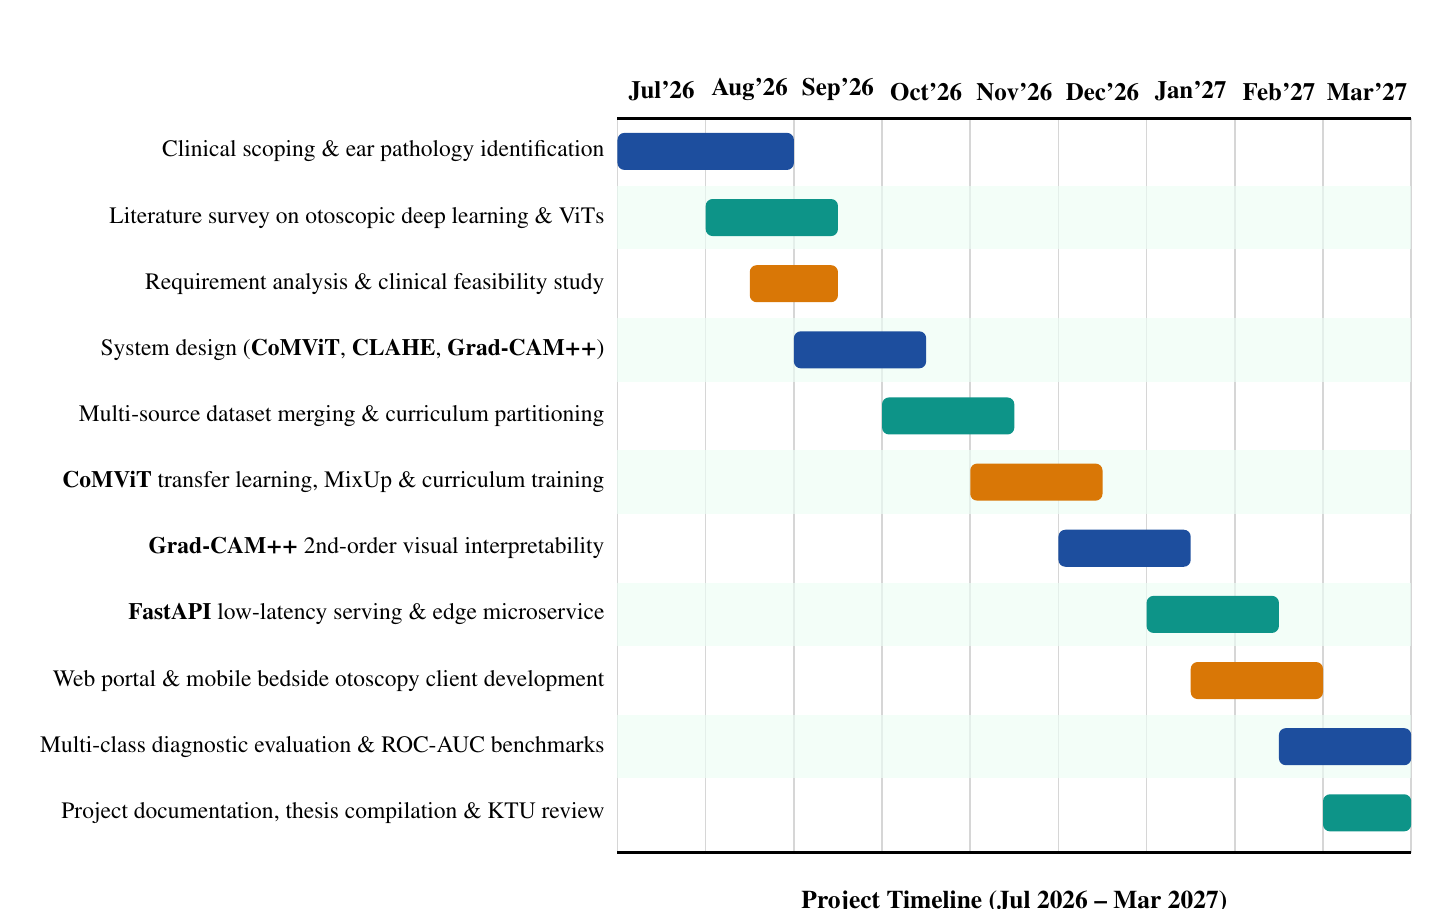
\begin{tikzpicture}[
  x=1.12cm, y=0.84cm,
  lab/.style={anchor=east, font=\fontsize{8.5}{10.5}\selectfont, inner sep=4.5pt, text=black}
]
\def\nm{9}
\def\topY{11.5}

% Vertical month gridlines
\foreach \i in {0,1,...,\nm} {
  \draw[gray!32, line width=0.55pt] (\i, 0.4) -- (\i, \topY);
}

% Month headers on top
\foreach \i/\m in {0.5/Jul'26, 1.5/Aug'26, 2.5/Sep'26, 3.5/Oct'26, 4.5/Nov'26, 5.5/Dec'26, 6.5/Jan'27, 7.5/Feb'27, 8.5/Mar'27} {
  \node[anchor=south, font=\fontsize{9.0}{11.0}\selectfont\bfseries, text=black] at (\i, \topY+0.12) {\m};
}
\draw[black, line width=1.0pt] (0, \topY) -- (\nm, \topY);
\draw[black, line width=0.8pt] (0, 0.4) -- (\nm, 0.4);

% Alternating row background shading
\foreach \k in {0,...,10} {
  \pgfmathsetmacro{\yc}{11.0-\k}
  \ifodd\k
    \fill[prismMint, opacity=0.65] (0, \yc-0.48) rectangle (\nm, \yc+0.48);
  \fi
}

% Task milestone labels on left
\node[lab] at (0, 11.0) {Clinical scoping \& ear pathology identification};
\node[lab] at (0, 10.0) {Literature survey on otoscopic deep learning \& ViTs};
\node[lab] at (0, 9.0)  {Requirement analysis \& clinical feasibility study};
\node[lab] at (0, 8.0)  {System design (\textbf{CoMViT}, \textbf{CLAHE}, \textbf{Grad-CAM++})};
\node[lab] at (0, 7.0)  {Multi-source dataset merging \& curriculum partitioning};
\node[lab] at (0, 6.0)  {\textbf{CoMViT} transfer learning, MixUp \& curriculum training};
\node[lab] at (0, 5.0)  {\textbf{Grad-CAM++} 2nd-order visual interpretability};
\node[lab] at (0, 4.0)  {\textbf{FastAPI} low-latency serving \& edge microservice};
\node[lab] at (0, 3.0)  {Web portal \& mobile bedside otoscopy client development};
\node[lab] at (0, 2.0)  {Multi-class diagnostic evaluation \& ROC-AUC benchmarks};
\node[lab] at (0, 1.0)  {Project documentation, thesis compilation \& KTU review};

% Milestone Gantt Bars
\fill[prismBlue, rounded corners=2.5pt]     (0.0, 11.0-0.28) rectangle (2.0, 11.0+0.28);
\fill[prismTeal, rounded corners=2.5pt]     (1.0, 10.0-0.28) rectangle (2.5, 10.0+0.28);
\fill[prismGold, rounded corners=2.5pt]     (1.5, 9.0-0.28)  rectangle (2.5, 9.0+0.28);
\fill[prismBlue, rounded corners=2.5pt]     (2.0, 8.0-0.28)  rectangle (3.5, 8.0+0.28);
\fill[prismTeal, rounded corners=2.5pt]     (3.0, 7.0-0.28)  rectangle (4.5, 7.0+0.28);
\fill[prismGold, rounded corners=2.5pt]     (4.0, 6.0-0.28)  rectangle (5.5, 6.0+0.28);
\fill[prismBlue, rounded corners=2.5pt]     (5.0, 5.0-0.28)  rectangle (6.5, 5.0+0.28);
\fill[prismTeal, rounded corners=2.5pt]     (6.0, 4.0-0.28)  rectangle (7.5, 4.0+0.28);
\fill[prismGold, rounded corners=2.5pt]     (6.5, 3.0-0.28)  rectangle (8.0, 3.0+0.28);
\fill[prismBlue, rounded corners=2.5pt]     (7.5, 2.0-0.28)  rectangle (9.0, 2.0+0.28);
\fill[prismTeal, rounded corners=2.5pt]     (8.0, 1.0-0.28)  rectangle (9.0, 1.0+0.28);

% Bottom title
\node[font=\fontsize{9.2}{11.2}\selectfont\bfseries, text=black] at (4.5, -0.35) {Project Timeline (Jul 2026 -- Mar 2027)};
\end{tikzpicture}
\end{document}
}
    \caption{Project execution schedule and Gantt chart tracking 11 key milestones from July 2026 to March 2027.}
    \label{fig:project_gantt}
\end{figure}

The eleven coordinated work packages executed across the academic timeline were:
\begin{enumerate}
    \item \textbf{Clinical Scoping \& Problem Identification (Jul--Aug 2026):} Defined screening boundaries, clinical triage workflows, and ear disease diagnostic requirements.
    \item \textbf{Literature Survey on Otoscopic Deep Learning \& ViTs (Aug--Sep 2026):} Reviewed CNN architectures, Vision Transformers, domain generalization, and XAI methods.
    \item \textbf{Requirement Analysis \& Clinical Feasibility Study (Aug--Sep 2026):} Compiled functional and non-functional specifications and safety bounds.
    \item \textbf{System Design (CoMViT, CLAHE, Grad-CAM++) (Sep--Oct 2026):} Architected the multi-tier system, component dataflows, and relational schemas.
    \item \textbf{Multi-Source Dataset Merging \& Curriculum Partitioning (Oct--Nov 2026):} Curated multi-source otoscopic corpora, filtered corrupt files, and split 70/15/15.
    \item \textbf{CoMViT Transfer Learning, MixUp \& Curriculum Training (Nov--Dec 2026):} Implemented AdamW optimization, controlled MixUp, and adaptive curriculum training.
    \item \textbf{Grad-CAM++ 2nd-Order Visual Interpretability (Dec 2026--Jan 2027):} Hooked terminal transformer block and engineered Jet colormap overlay synthesis.
    \item \textbf{FastAPI Low-Latency Serving \& Edge Microservice (Jan--Feb 2027):} Developed asynchronous REST endpoints with MIME and payload validation.
    \item \textbf{Web Portal \& Mobile Bedside Otoscopy Client Development (Jan--Feb 2027):} Created clinical web dashboard and mobile digital otoscope scanner.
    \item \textbf{Multi-Class Diagnostic Evaluation \& ROC-AUC Benchmarks (Feb--Mar 2027):} Evaluated 1,250 test images, achieving 95.44\% accuracy and 98.85\% ROC-AUC.
    \item \textbf{Project Documentation, Thesis Compilation \& KTU Review (Feb--Mar 2027):} Compiled comprehensive project report and thesis documentation.
\end{enumerate}


%==============================================================================
% CHAPTER 9: CONCLUSION AND FUTURE SCOPE
%==============================================================================
\chapter{Conclusion and Future Scope}

\section{Conclusion}
This project successfully designed, implemented, and empirically evaluated an automated, interpretable deep learning framework for \textbf{Ear Disease Detection from Otoscopic Images Using Robust Deep Learning Models}. Addressing the clinical challenges of non-specialist diagnostic error, ENT specialist shortages, domain shift across diverse otoscope hardware, and black-box opacity, the framework establishes an accurate, robust, and explainable preliminary screening platform.

The core diagnostic engine leverages \textbf{CoMViT}, an efficient Vision Transformer architecture that captures both fine local eardrum textures and global tympanic membrane context across five target classes: \textbf{Acute Otitis Media (AOM)}, \textbf{Chronic Suppurative Otitis Media (CSOM)}, \textbf{Earwax}, \textbf{Normal}, and \textbf{Tympanosclerosis}. Generalization is enforced via \textbf{Contrast Limited Adaptive Histogram Equalization (CLAHE)}, \textbf{online data augmentation}, \textbf{controlled MixUp augmentation}, and \textbf{adaptive curriculum learning}. To establish clinical trust, \textbf{Grad-CAM++} utilizes second-order partial derivatives to generate high-resolution visual heatmaps localizing authentic pathological features on the tympanic membrane.

Empirical evaluation on an independent benchmark of 1,250 clinical otoscopic images demonstrated outstanding performance, achieving an overall accuracy of \textbf{95.44\%}, a macro F1-score of \textbf{95.49\%}, and an ROC-AUC of \textbf{98.85\%}. Deployed via an asynchronous \textbf{FastAPI} microservice delivering sub-50ms inference alongside responsive web and mobile digital otoscope clients, the framework establishes a practical, point-of-care clinical decision-support tool.

\section{Limitations Encountered}
Despite the strong empirical results, certain clinical and operational limitations remain:
\begin{itemize}
    \item \textbf{Total Cerumen Occlusion:} Severe impacted earwax completely blocks visualization of the tympanic membrane, preventing assessment of underlying middle ear infections until manual earwax removal is performed.
    \item \textbf{Static 2D Snapshot Constraints:} Static photographs cannot assess dynamic tympanic membrane mobility, which in clinical practice is evaluated using pneumatic otoscopy.
    \item \textbf{Subtle Early Myringitis:} Very early stages of viral myringitis with minimal vascular injection can occasionally present diagnostic ambiguity against normal variants.
\end{itemize}

\section{Future Scope}
Promising directions for future research and engineering enhancements include:
\begin{itemize}
    \item \textbf{Video Otoscopy and Temporal Frame Aggregation:} Extending CoMViT with recurrent or spatio-temporal attention to analyze continuous digital otoscope video streams, automatically selecting optimal focal frames.
    \item \textbf{Direct On-Device Edge Deployment:} Quantizing CoMViT using TensorRT and INT8 precision for direct deployment on low-cost single-board computers (such as Rockchip RK3566 or Raspberry Pi) inside handheld otoscope handles.
    \item \textbf{Federated Multi-Hospital Learning:} Implementing privacy-preserving federated learning protocols enabling model parameter updates across distributed hospitals without transferring private patient otoscopic data.
    \item \textbf{Tympanometry Multi-Modal Fusion:} Fusing otoscopic visual features with acoustic impedance tympanometry graphs to provide comprehensive multi-modal middle ear diagnostics.
\end{itemize}


%==============================================================================
% REFERENCES
%==============================================================================
\begin{thebibliography}{99}
\sloppy

\bibitem{ref_hayashi2020_aom}
T.~Hayashi, K.~Kitamura, S.~Hashimoto, M.~Hotomi, H.~Kojima, F.~Kudo, Y.~Maruyama, S.~Sawada, H.~Taiji, G.~Takahashi, H.~Takahashi, Y.~Uno, and H.~Yano, ``Clinical practice guidelines for the diagnosis and management of acute otitis media in children---2018 update,'' \textit{Auris Nasus Larynx}, vol.~47, no.~4, pp.~493--526, 2020.

\bibitem{ref_abuzinadah2026_attention}
H.~Abu-Zinadah and S.~Abdel-Khalek, ``Mathematical modeling and feature extraction architecture of a quantum-inspired attention network for UAV image classification,'' \textit{Alexandria Engineering Journal}, vol.~143, pp.~180--193, 2026.

\bibitem{ref_mahdiani2021_csom}
S.~Mahdiani, L.~Lasminingrum, and D.~Anugrah, ``Management evaluation of patients with chronic suppurative otitis media: A retrospective study,'' \textit{Annals of Medicine and Surgery}, vol.~67, art.~102492, pp.~1--5, 2021.

\bibitem{ref_aburass2025_vit}
S.~Aburass, O.~Dorgham, J.~Al~Shaqsi, M.~Abu~Rumman, and O.~Al-Kadi, ``Vision Transformers in medical imaging: A comprehensive review of advancements and applications across multiple diseases,'' \textit{Journal of Imaging Informatics in Medicine}, vol.~38, no.~5, pp.~3928--3971, 2025.

\bibitem{ref_kitaguchi2026_gradcampp}
Y.~Kitaguchi, Y.~Ueno, T.~Yamaguchi, H.~Maehara, D.~Miyazaki, R.~Nejima, T.~Inomata, N.~Kato, T.~Chikama, J.~Ominato, T.~Yunoki, K.~Tsubota, M.~Oda, K.~Mori, Y.~Yoshinaga, R.~Iwasaki, K.~Nishida, and T.~Oshika, ``YOLOv5 attention analysis for anterior eye disease classification: Grad-CAM++ feature importance and cut-and-paste validation,'' \textit{Journal of Imaging Informatics in Medicine}, vol.~39, no.~4, pp.~3340--3355, 2026.

\bibitem{ref_cha2019_ensemble}
D.~Cha, C.~Pae, S.-B. Seong, J.~Y. Choi, and H.-J. Park, ``Automated diagnosis of ear disease using ensemble deep learning with a big otoendoscopy image database,'' \textit{EBioMedicine}, vol.~45, pp.~606--614, 2019.

\bibitem{ref_habib2022_ai_otoscopy}
A.-R. Habib, M.~Kajbafzadeh, Z.~Hasan, E.~Wong, H.~Gunasekera, C.~Perry, R.~Sacks, A.~Kumar, and N.~Singh, ``Artificial intelligence to classify ear disease from otoscopy: A systematic review and meta-analysis,'' \textit{Clinical Otolaryngology}, vol.~47, no.~3, pp.~401--413, 2022.

\bibitem{ref_lindmark2024_generalizable}
M.~Lindmark, T.~Lundberg, M.~Werner, P.~Soda, C.~Gr{\"o}nlund, and F.~{\"O}hberg, ``Towards generalizable image classification models for detecting middle ear diseases,'' \textit{IEEE Access}, vol.~12, pp.~37239--37253, 2024.

\bibitem{ref_nemati2021_tympanosclerosis}
S.~Nemati, A.~Saberi, A.~F. Habibi, H.~Hemmati, R.~Jafari-Shakib, M.~H. Ch, and E.~Bozorgzadeh, ``Tympanosclerosis and atherosclerosis plaques: A comparative analytical study on some new microbiological and immunohistochemical aspects,'' \textit{European Archives of Oto-Rhino-Laryngology}, vol.~278, no.~8, pp.~2805--2812, 2021.

\bibitem{ref_yang2026_otitis}
C.-Y. Yang, C.-J. Lee, W.-S. Lai, K.-Y. Chen, C.-F. Kuo, C.~H. Liu, and S.-C. Liu, ``Deep learning-based semantic segmentation and classification of otoscopic images for otitis media diagnosis and health promotion,'' \textit{Diagnostics}, vol.~16, no.~3, art.~467, pp.~1--12, 2026.

\bibitem{ref_gao2023_augmented_gradcampp}
Y.~Gao, J.~Liu, W.~Li, M.~Hou, Y.~Li, and H.~Zhao, ``Augmented Grad-CAM++: Super-resolution saliency maps for visual interpretation of deep neural network,'' \textit{Electronics}, vol.~12, no.~23, art.~4846, pp.~1--23, 2023.

\bibitem{ref_van2025_tympanosclerosis}
S.~Van, D.~{\"O}zdemir, S.~K. {\c{S}}ahin, {\c{S}}.~{\"O}zt{\"u}rk, D.~M. Mehel, and A.~{\c{C}}e{\c{c}}en, ``The role of matrix metalloproteinase expression levels in the pathogenesis of tympanosclerosis,'' \textit{European Archives of Oto-Rhino-Laryngology}, vol.~282, no.~11, pp.~5645--5653, 2025.

\bibitem{ref_yokananth2025_otovision}
R.~Yokananth and V.~Gosula, ``OtoVision: Bridging machine learning and edge computing for effective and affordable ear disease diagnosis,'' \textit{Neural Computing and Applications}, vol.~37, no.~3, pp.~1565--1573, 2025.

\bibitem{ref_demircan2025_attention}
F.~Demircan, M.~Ekinci, and Z.~C{\"o}mert, ``Enhancing intra-aural disease classification with attention-based deep learning models,'' \textit{Neural Computing and Applications}, vol.~37, no.~10, pp.~6601--6616, 2025.

\bibitem{ref_onifade2025_csom_prevalence}
A.~Onifade, H.~W. Katolo, S.~Mookerjee, and M.~F. Bhutta, ``Epidemiology of chronic suppurative otitis media: Systematic review to estimate global prevalence,'' \textit{Journal of Epidemiology and Global Health}, vol.~15, art.~55, pp.~1--12, 2025.

\bibitem{ref_dosovitskiy2020_vit}
A.~Dosovitskiy, L.~Beyer, A.~Kolesnikov, D.~Weissenborn, X.~Zhai, T.~Unterthiner, M.~Dehghani, M.~Minderer, G.~Heigold, S.~Gelly, J.~Uszkoreit, and N.~Houlsby, ``An image is worth 16x16 words: Transformers for image recognition at scale,'' in \textit{International Conference on Learning Representations (ICLR)}, 2021.

\bibitem{ref_zhang2017_mixup}
H.~Zhang, M.~Cisse, Y.~N. Dauphin, and D.~Lopez-Paz, ``mixup: Beyond empirical risk minimization,'' in \textit{International Conference on Learning Representations (ICLR)}, 2018.

\bibitem{ref_bengio2009_curriculum}
Y.~Bengio, J.~Louradour, R.~Collobert, and J.~Weston, ``Curriculum learning,'' in \textit{Proceedings of the 26th Annual International Conference on Machine Learning (ICML)}, pp.~41--48, 2009.

\bibitem{ref_chattopadhay2018_gradcampp}
A.~Chattopadhay, A.~Sarkar, P.~Howlader, and V.~N. Balasubramanian, ``Grad-CAM++: Generalized gradient-based visual explanations for deep convolutional networks,'' in \textit{IEEE Winter Conference on Applications of Computer Vision (WACV)}, pp.~839--847, 2018.

\bibitem{ref_reza2004_clahe}
A.~M. Reza, ``Realization of the contrast limited adaptive histogram equalization (CLAHE) for real-time image enhancement,'' \textit{Journal of VLSI Signal Processing Systems for Signal, Image and Video Technology}, vol.~38, no.~1, pp.~35--44, 2004.

\bibitem{ref_selvaraju2017_gradcam}
R.~R. Selvaraju, M.~Cogswell, A.~Das, R.~Vedantam, D.~Parikh, and D.~Batra, ``Grad-CAM: Visual explanations from deep networks via gradient-based localization,'' in \textit{IEEE International Conference on Computer Vision (ICCV)}, pp.~618--626, 2017.

\end{thebibliography}

\end{document}
